
\documentclass[withoutpreface,bwprint]{cumcmthesis} %去掉封面与编号页
\usepackage{amsmath}
\usepackage{subeqnarray}
\usepackage{cases}

\usepackage{fontspec}
\usepackage{listings}


    \title{基于贪心算法和变步长搜索的“FAST”主动反射面的形状调节}
    \begin{document}
        \maketitle
        \begin{abstract}
          
"FAST"射电望远镜是我国自主研发的大国重器,在探测外太空,发现域外文明等天文
领域具有重要意义,本文主要讨论了"FAST"的主动反射形状调节,并给出了能较大提升馈源舱接收率的调整方案。 


 针对问题1,为了求得在$\alpha=0^\circ,\beta = 90^\circ $时的理想抛物面,我们以C为球心,竖直方向为z轴,
 水平方向为x轴建立空间直角坐标系,然后将三维问题转化为二维平面内进行简化分析,
 接着基于两种调节策略——建立了理想抛物面的优化模型,通过变步长搜索,经过粗搜索和细搜索过程
 最终得到了径向差值的分布曲线,并求得抛物面顶点与直线SC交于基准圆球的交点间的距离h为0.397m,并基于建立的坐标系
 得到了理想抛物面方程为:
 $-(x^2+y^2)+559.2z+167982.0024 =0\quad$.
 

 针对问题2, 基于问题1的模型建立求解过程,为了求得在$\alpha = 36.795^\circ , \beta = 78.169^\circ$时的理想抛物面
 问题2首先进行了坐标系的变换,乘以旋转矩阵后消除了天体带来的角度差异,通过简单的计算排除抛物面超出圆周边界的可能后,
 根据问题1相同的步骤,求得抛物面顶点与直线SC交于基准圆球的交点间的距离h为0.377m,再经过反旋转后得到了原坐标系的理想抛物面的方程为
 $167971 - 0.973045 x^2 - 0.984919 y^2 + y (68.671 + 0.240387 z)+ x (91.8091 + 0.0403239 y + 0.321384 z)+ 547.321 z - 0.0420355 z^2 = 0$,
 并验证了结果的正确性。第二部分为了建立使基准球面尽可能贴近抛物面的调整模型,在查阅文献后构建了基于曲面平均曲率的调整模型,并结合第三问对其进行了参数搜索,得到的调整方案
对口径内的主索节点调整距离大多在[0,0.6]内,其中有接近1/3为0.6左右, 将结果存入了resulx.xlsx文件中。然后对调整后主索节点间的微小波动(附录条件5)也予以了讨论,发现主索节点的波动相比于调整距离
较大,可能会对调整方案产生影响,具体研究了在波动发生率为20\%的情况下主索节点的波动情况,发现部分主索节点调整距离发生了[-0.16648m,+0.16648m]范围内的偏移。





 针对问题3,为了求取照明区域内被馈源舱接收的有效信号与总入射信号的比值,
 我们将其转化为有效反射信号对应的反射面板在以入射信号为法向量投影平面的总投影面积与照明区域总投影面的比值。
 然后从单个三角面板进行分析,在已有的三维坐标系下建立了三角反射面板的反射模型,
 根据附件一种反射面板三点坐标等相关信息计算出反射面板投影面积,反射面方程与入射信号方程,
 并求解出反射信号与馈源舱所在平面交点,判断出落在馈源舱接受区域的反射信号并获取对应反射面板投影面积,
 将所有有效投影面积累加最后计算出基准反射球面接受比为11.3\%,调整后馈源舱接受比为65.9\%,
 信号接收比有较大提升,方案实际调整效果较好。





            \keywords{贪心算法\quad  变步长搜索  \quad  坐标变换}
        \end{abstract}


        \section{问题重述}

   问题提出:本文主要研究的是"FAST"球面射电望远镜的反射面板调节策略,其中主要涉及到了关于立体几何,光学等知识,
   由于抛物面具有的汇光特性,可将平行光汇聚于一点以此被馈源舱接受,经过分析而显示出远处的天体,以此达到望远效果。
   但由于本身望远镜是球面,只能获得线状反射光,所以巧妙地利用反射面板调节计数近似瞬时工作抛物面。

   问题1 : 问题1需要我们研究位于基准球面正上方即(即$\alpha=0^\circ,\beta = 90^\circ $)
   时,考虑反射面板的径向调节距离在$[-0.6,0.6]$这个限制,来确定理想抛物面。

     问题2:  问题2分为两小问,第一小问与问题1类似先要求我们确定当天体S的方位角位于$\alpha = 36.795^\circ , \beta = 78.169^\circ$
     时的理想抛物面,第二小问要求我们根据所有求得的理想抛物面,确定反射面板的调节模型,来让反射面尽量贴近理想抛物面。 

     
问题3:问题3需要我们考虑不进行调整和进行问题2中的调整方案后的馈源舱接收电磁波的比例,并进行比较。


        \section{问题分析}
            本问题中原有的基准球面只能将平行光线汇聚成线状,而抛物面能确保所有平行光线汇聚于焦点,使得光线都能落在馈源舱的有效区域内,
        因此需要调节反射面板合成近似抛物面。
    
		\subsection{问题1}

        问题1需要求解当待观测天体位于基准球面正上方时的理想抛物面的位置,而确定理想抛物面不仅仅需要考虑焦距的因素,
        也需要考虑反射面板调节因素,根据每个促动器的调节范围[-0.6m,0.6m]
        来进行设计。以球心C为原点,竖直方向为z轴,水平方向为y轴,建立笛卡尔坐标系(右手系),首先由于观测天体在基准球面的正上方,
        因此旋转抛物面的顶点就可以安排在z轴上,根据题目中给予的焦径比,也使得当旋转抛物面的口径与基准球半径相等且抛物面顶点
        位于基准球面上时,旋转抛物面正好交于基准球内,又根据基准球面和基准抛物面各向同性的特点,可以简化
        三维模型至二维平面内,将球简化成圆,抛物面简化成抛物线分析,根据焦径比计算得出抛物线的焦距后,只需要确定顶点的高度就可以
        得到理想抛物线方程,最后由于围绕z轴旋转一周即可得到理想旋转抛物面方程。
        
        此题的天体位置大大简化了模型,问题的重点就在于抛物面顶点的高度,可以根据两个指标来选择合适的高度,通过文献查阅后,
	    了解到fast主索网需要减小主索节点的经向位移,避免变形后主索发生松弛,在基准球面状态时,若经向位移过大就要加大主索预应力值$^[1]$,
	    这样使主索单元疲劳性加大,降低索网运行的可靠性,因此需要考虑以下两种策略,分别是主索节点的总位移最小,抛物面弧长与球面弧长差最小,
	    在满足主索节点的限制条件和反射效率最大化的前提下,问题就转换为抛物面顶点和基准球面对应顶点间距离的优化问题,具体求解见后文。
        
        
        
        \subsection{问题2}

        问题2主要分为两个部分,首先求解观测天体$S$位于$\alpha = 36.795^\circ, \beta = 78.169^\circ$时理想抛物面的位置和
        调节反射面板来近似理想抛物面的调解方案。针对第一部分,由于天体方位产生了变化,我们考虑进行坐标系的转,将实际坐标系
        乘以对应的旋转矩阵转换到同问题1的坐标系中,这样可以简化分析。利用问题1的求解方法,我们可以得到旋转坐标系中的理想抛物线
        方程,将抛物线绕对称轴旋转一周后,再进行坐标反变换,最终可以得到在原有坐标系中的理想旋转抛物面方程。

        针对第二部分,需要由实际的三角球形反射面板去尽可能地贴近理想抛物面,将问题同样转化到二维分析后,我们考虑了两种优化模型
        来衡量实际抛物面与理想抛物面的差异,最终设想通过第三问的接受比来选择一种更优的模型。主要的限制条件其实就在于促动器伸缩的限制,也即主索节点的伸缩限制。而在实际调节反射面板
        的过程中,我们还不能忽略附录5中所提到的当主索节点沿着径向移动时,节点间距离的微小变化,将这一0.07\%的变化作为均匀分布的误差
        代入模型的求解算法中,也会对结果产生一定影响,因此也需要加以考虑。对于该问题的求解算法,本文中采用的是基于赋权无向图的贪心算法,
        因此是从一个特定点开始对于相邻的主索节点一个个调节的,具体的求解见后文。
        
        
        \subsection{问题3} 
        问题3要求我们计算出在调整反射面板前后馈源舱的接收比,以此来分析问题2中方案的实际调整效果。这是一个物理光学反射问题,
        需要对每一块反射面板建立数学模型进行分析,在已知反射面板坐标,入射点与入射方向情况下求出反射面与入射信号的方程,
        进而求解出反射光线与馈源舱平面的交点,并判断反射信号是否被馈源舱捕获。
        最后考虑将有效反射信号对应的反射板面积累加并与总接收面积进行比值求解出接收比,
        并将调整前后接收比进行对比以分析问题2中的方案的好坏。









        \section{问题假设}
        \begin{itemize}
            \item  1:假设天体S离fast射电望远镜足够远,射电望远镜口径与此距离相比可以忽略不计,此时来自天体S的电磁波可视为平行射入。
            \item  2:假设天体半径与天体到fast射电望远镜的距离相比可以忽略不计。 
            \item  3:假设反射面板无孔。(透水孔小于电磁波长)
            \item  4:假设到达馈源舱的光线就能被馈源舱所接受,不考虑光强大小。
        \end{itemize}
        

        
        \section{符号假设}

        \begin{longtable}{p{8cm}<{\centering}p{7.5cm}}
            \toprule  %添加表格头部粗线
            符号& 意义\\
            \midrule  %添加表格中横线
            $h$ & 抛物面顶点到基准球面间的距离  \\
            $R$  & 基准球面半径\\
            $f$   &焦径比\\
            $D$   &抛物面口径\\
            $\Delta$ & 近似径向位移差\\
            $V_s$ & 起始搜索点\\
            $V_i$ &第i个搜索点(主索节点)\\
            $x_{v_i}$ &第i个搜索点的x坐标\\
            $y_{v_i}$ &第i个搜索点的x坐标\\
            $z_{v_i}$ &第i个搜索点的x坐标\\
            $d_{MaxAdjustUp_i}$&第i个搜索节点的最大正调节距离\\
            $d_{MaxAdjustLower_i}$&第i个搜索节点的最大负调节距离\\
            $d_i$ &第i个节点的调节距离 \\
            $a_i$ & 第i块面板反射信号落在馈源舱情况\\
            $b_i$ & 第i块面板反射信号落在照明区域情况\\
            $S_i$ & 第i块反射面板投影面积\\
            $\omega$ & 接收比\\
            \bottomrule %添加表格底部粗线
        \end{longtable}

        \newpage


        \section{模型求解}

        \subsection{问题1}

        \subsubsection{模型准备}
将附件1中的所有主索节点的坐标画出散点图,并根据附件1提取出300m口径内的主索节点,总数为1179个,得到分布情况大致如下,
下图中绿色点代表在口径300m内的主索节点:

\begin{figure}[H]
    \begin{minipage}[t]{0.5\linewidth}
    \centering
    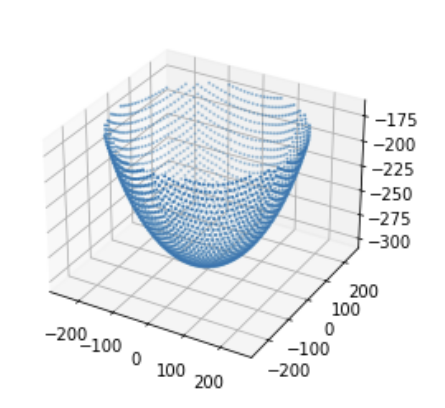
\includegraphics[scale=0.5]{images/allsuo.png}
    \caption{主索节点分布图}
    \label{fig:side:c}
    \end{minipage}%
    \begin{minipage}[t]{0.5\linewidth}
    \centering
    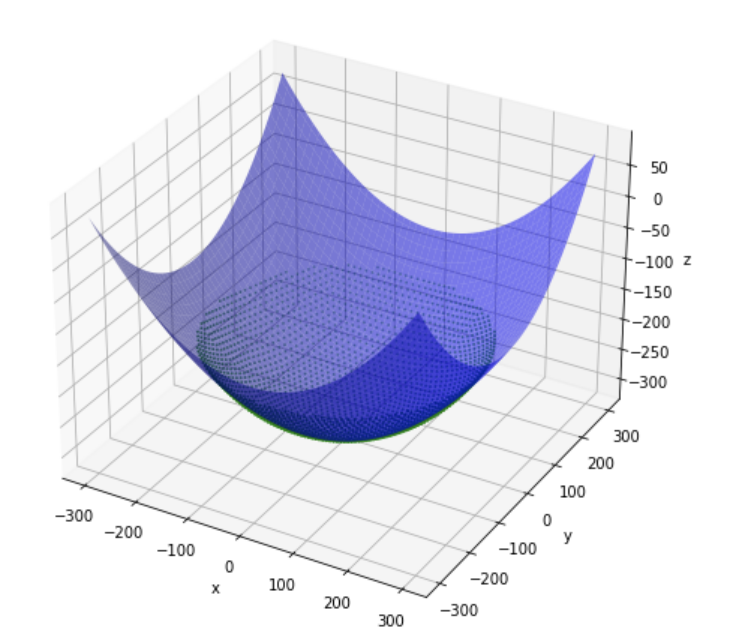
\includegraphics[scale=0.35]{images/zhunbei2.png}
    \caption{300m口径内主索节点分布图}
    \label{fig:side:d}
    \end{minipage}
\end{figure}

        \subsubsection{模型建立}

        正因为观测天体$S$位于基准球面正上方,可得到焦点即为直线SC与焦面的交点$P$,建立直角坐标系如下图:
        \begin{figure}[H]
    
            \centering
            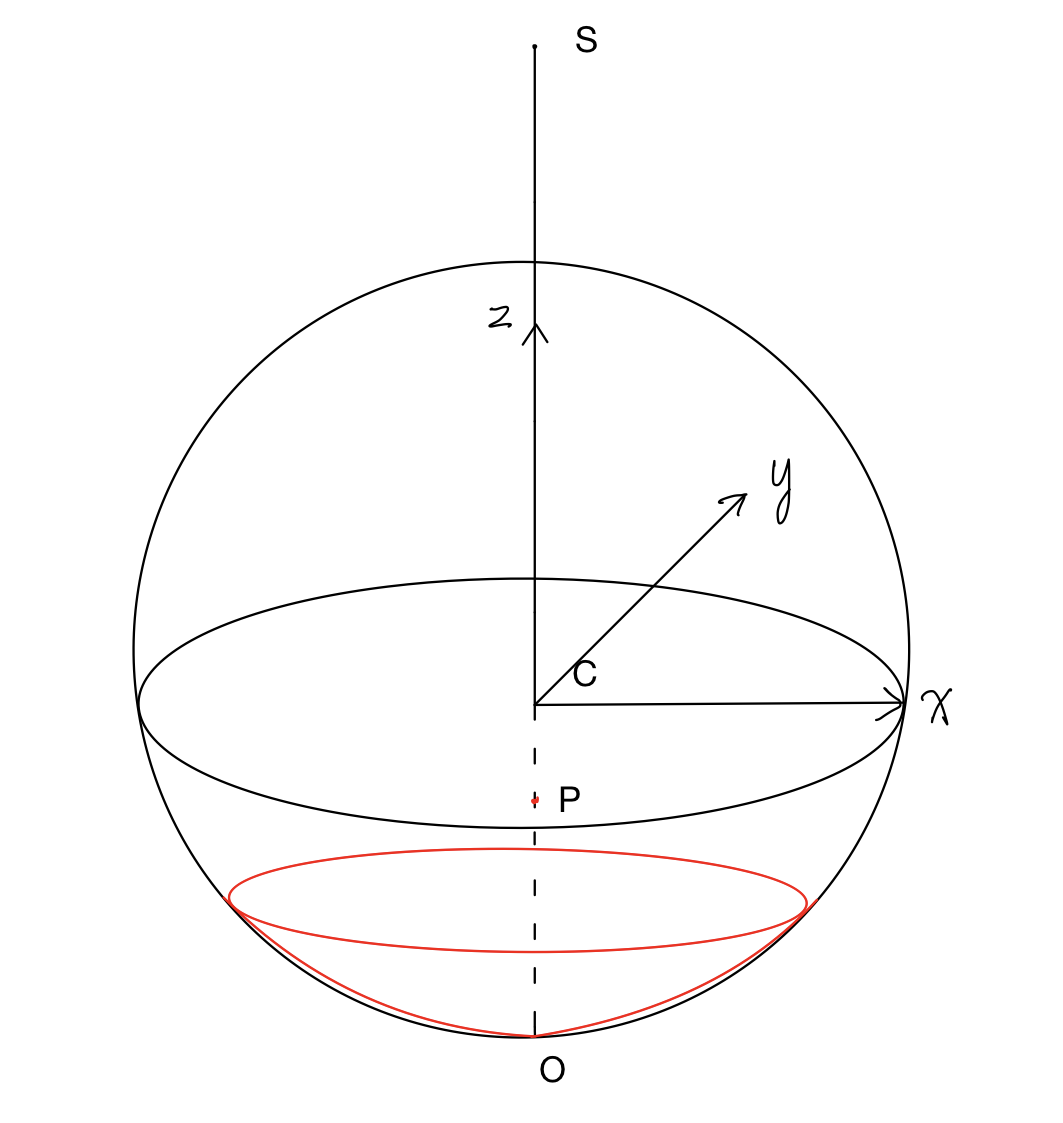
\includegraphics[scale=0.26]{images/zuobiaoxi.png}
            \caption{世界坐标系}
        \end{figure}

        球面和抛物面都具有各向同性特点,所以分析变形策略时,可以将问题简化到二维空间,用圆弧线替代基本球面、抛物线替代抛物面,
        分析剖面来简化原有问题。
        现以基准球面球心为坐标原点,圆弧和抛物线方程如下,球面半径(R = 300 m)与抛物面口径相等
        则对应的圆方程(1) 和抛物线方程如下:
        \begin{subequations}  
            \begin{numcases}{} 
                x^2+y^2=R^2\quad \\ 
                -x^2+4Dfy+4Df(R+h) =0\quad
            \end{numcases} 
        \end{subequations}

        示意图如下:
        \begin{figure}[H]
    
            \centering
            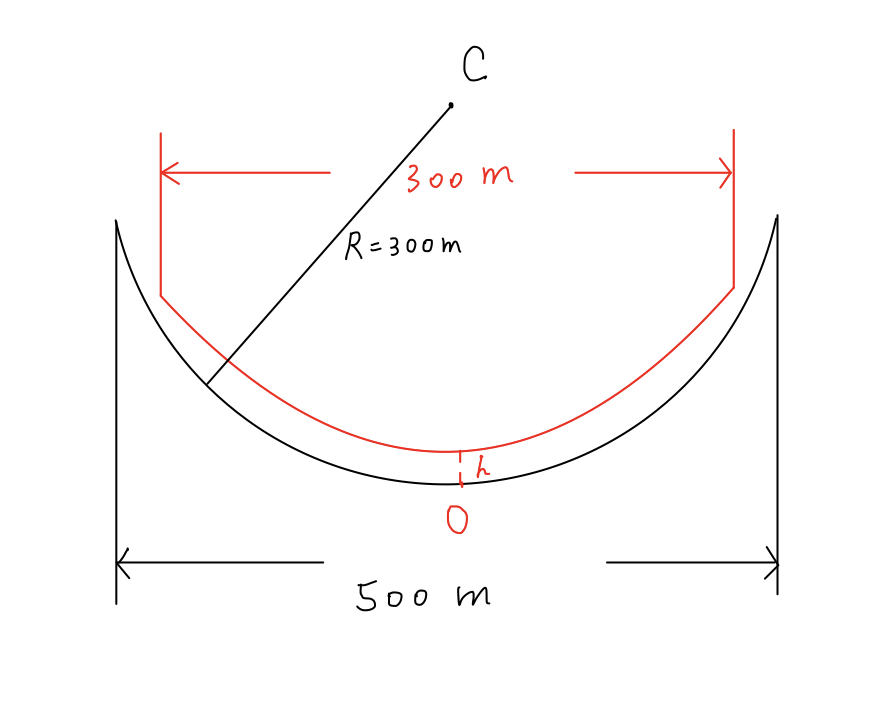
\includegraphics[scale=0.5]{images/shiyi.png}
            \caption{二维平面分析示意图}
        \end{figure}


其中$R$为基准球面半径$R=300m$,$D$为抛物面口径$D=300m$,$h$是抛物面顶点到基准球面间的距离,$f$为焦径比$\frac{F}{R}$,
题干中已给出:$f=0.466$,此时抛物线的焦距为:$fD =fR=F$,此时由于抛物线的汇聚性质,所有的入射平行
电磁波都会被聚集在馈源舱。此时理想的吸收率为100\%.
    
则在问题1中$ \alpha = 0^\circ ,\beta = 90^\circ$ 时,考虑反射面板调节因素的限制,在口径300m拟合最优抛物线即为理想抛物线。

考虑到主索节点伸缩范围的限制条件,因为题目的特殊性,所以有 $−0.6m≤h≤0.6m $,在此基础下,考虑反射面板调节范围限制因素、拉索所受应力
等因素,同时又要便于之后的主索节点进行调节,我们把问题转化成优化问题,并关注以下优化目标$^{[2]}$:

(1) 主索节点径向位移最小;

(2) 抛物面弧长与球面弧长差最小;


\hspace*{\fill}

\hspace*{\fill}

(1)考虑主索节点的位移: 
对于每个特定的h,为了表征300m口径内的主索节点的位移,考虑$[-150m,150m]$内每个节点的与抛物线在该点处的径向位移差,
为了表示方便,我们采用极坐标,以C为原点,与x轴的夹角$\theta$建立极坐标系,逆时针为正向:

即考虑$\theta\in [-\frac{2\pi}{3},-\frac{\pi}{3}]$内的情况,下图以$h=0$为例:


\begin{figure}[H]
    \centering
    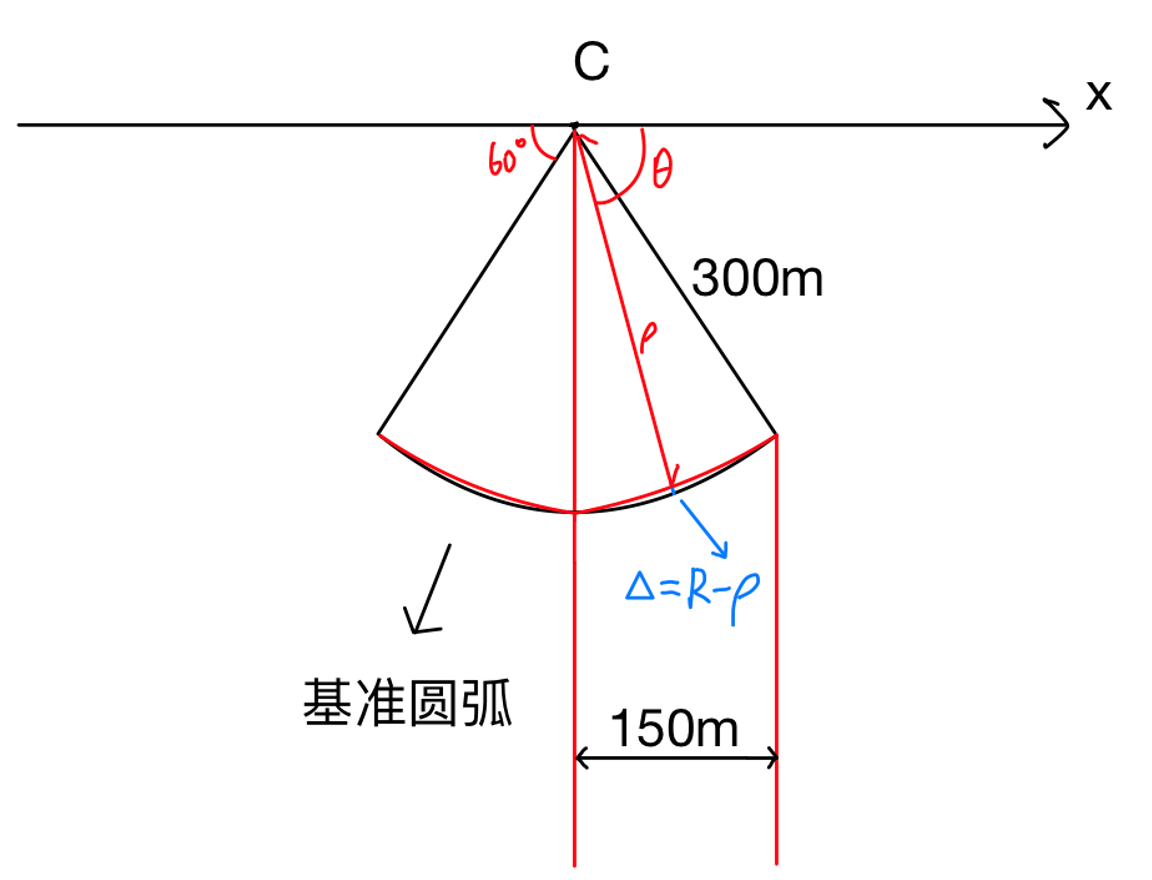
\includegraphics[scale=0.25]{images/jizuobiao.png}
    \caption{极坐标系示意图}
\end{figure}


此时,两者极坐标方程为:
\begin{subequations}  
    \begin{numcases}{} 
        \rho = R \\
    4Df(\rho \sin\theta +R+h)=\rho^2\cos^2\theta
    \end{numcases} 
\end{subequations}


由于此问题求解的是理想抛物面,虽然$\rho-R$本身不一定是外圆弧的径向,但从图中看出两者差距非常微小,可大致近似为
径向移动差值。

由于指向圆心方向为促动器伸缩正方向,因而可得到两者径向差值为:
\begin{equation}
    \Delta = R - 2 \sec^2\theta (D f \sin\theta + \sqrt{ D f \cos^2 \theta (h + R + D f \tan^2 \theta)})
\end{equation}


为了满足主索节点伸缩范围的限制条件,那么
\begin{equation}
     -0.6\leq \Delta \leq0.6,\quad  \forall  \theta\in [-\frac{2\pi}{3},-\frac{\pi}{3}] 
\end{equation}




正因为上述伸缩范围的限制条件,考虑到之后实际调节过程中需要使得实际近似抛物面贴近理想抛物面,我们尽量
让主索节点的径向位移总和尽可能小,便于之后反射面板调节的实现及优化,由此得到初步模型:

\begin{center}
    $Min \quad \sum \Delta^2 $

    $s.t  -0.6\leq \Delta \leq0.6,
    \quad  \forall  \theta\in [-\frac{2\pi}{3},-\frac{\pi}{3}]$
\end{center}


\hspace*{\fill}

\hspace*{\fill}

\hspace*{\fill}

(2) 抛物面弧长与球面弧长差最小;

由弧长公式可以计算得到在[-150,150]内:

圆的弧长: 

\begin{equation}
    l_c = \frac{\pi R}{3}
\end{equation}

抛物线的弧长:
\begin{equation}
    l_p = \int_{-\frac{D}{2}}^{\frac D 2}\sqrt{1+y^{\prime^2}} = \int_{-\frac{D}{2}}^{\frac D 2} \sqrt{1+\frac{x^2}{4D^2f^2}} = \frac{1}{ 8} D (\sqrt{16 + \frac{1}{f^2}} + 16 f arccsch(4 f))
\end{equation}

两者差为:
\begin{equation}
    l_{\Delta} = l_c-l_p =  \frac{\pi R}{3}- \frac{1}{ 8} D (\sqrt{16 + \frac{1}{f^2}} + 16 f arccsch(4f))
\end{equation}


为了尽可能拟合好,则两者差要尽可能小: 

即 
\begin{equation*}
    Min\quad  l_{\Delta} 
\end{equation*}

由于$l_{\Delta}$与搜索变量h无关,只与给出的f相关,所以可以用$l_{\Delta}$来检验题干焦径比对h搜索求解的影响,
带入f=0.466可得$l_{\Delta}=0.324517m$,也就是说在300m口径范围内,用基准圆来拟合抛物线只有0.324m的弧长差,
也就是0.1\%的误差,可以看出题干给出的焦径比搜索h可以得到一个拟合得很好的抛物面。


通过以上讨论,把问题1转化成以下规划问题:

\begin{equation*}
    Min \quad \sum \Delta^2
\end{equation*}


\begin{subequations}  
    \begin{numcases}{\text{$s.t$}} 
        -0.6\leq \Delta \leq0.6,\quad  \forall  \theta\in [-\frac{2\pi}{3},-\frac{\pi}{3}] \\ 
        -0.6\leq h\leq0.6
    \end{numcases} 
\end{subequations}


对于主索节点的位移的限制,由于模型为连续型模型,无法计算求解,所以对其进行离散化,取附件1中的x的所有坐标作为判断依据,
对其进行去重,并限制范围与300m口径内得到1179个不同的主索节点的横坐标,记其为$\{x_i\}$(i=1...1179)

则求解极坐标方程,代入最终得到求解理想抛物面的数学模型为:

\begin{equation*}
    Min \sum_{i=1}^{1179} \Delta_i^{2}
\end{equation*}


\begin{subequations}  
    \begin{numcases}{\text{$s.t$}} 
        -0.6\leq  \Delta_i \leq0.6,\quad  \forall  i = 1..1179 \\ 
        -0.6\leq h\leq0.6
    \end{numcases} 
\end{subequations}

其中,

\begin{align*}
    \theta &= -arccos\frac{x_i}{R}\\
    \Delta_i&=R-(2 \sec^2(-arccos\frac{x_i}{R}) (Df \sin(-arccos\frac{x_i}{R}) \\
    &- \sqrt{ D f \cos^2 (-arccos\frac{x_i}{R}) (h + R + D f \tan^2 (-arccos\frac{x_i}{R}))}
\end{align*}

\hspace*{\fill}

\hspace*{\fill}


\subsubsection{模型求解}

在求解模型之前,为了方便计算可以用数值求解软件Mathematics得到抛物线的数值解极坐标方程如下:

\begin{equation}
    \rho = 0.2(37.389838191679836\sqrt{2199+5h+801 \cos 2\theta+5h \cos2\theta}sec^2\theta+1398sec\theta tan\theta)
\end{equation}





随之对于上述优化问题,可将求解算法归结为以下步骤:

\textbf{$step1$}:首先进行粗搜索,以0.1m为步长搜索在h的取值范围$[-0.6,0.6]$内搜索h,得到一个较为粗糙的范围

在该粗搜索范围内,作出不同h对应的在口径300m内对应不同x坐标的理想抛物线与基准圆的径向差值:


\begin{figure}[H]
    \centering
    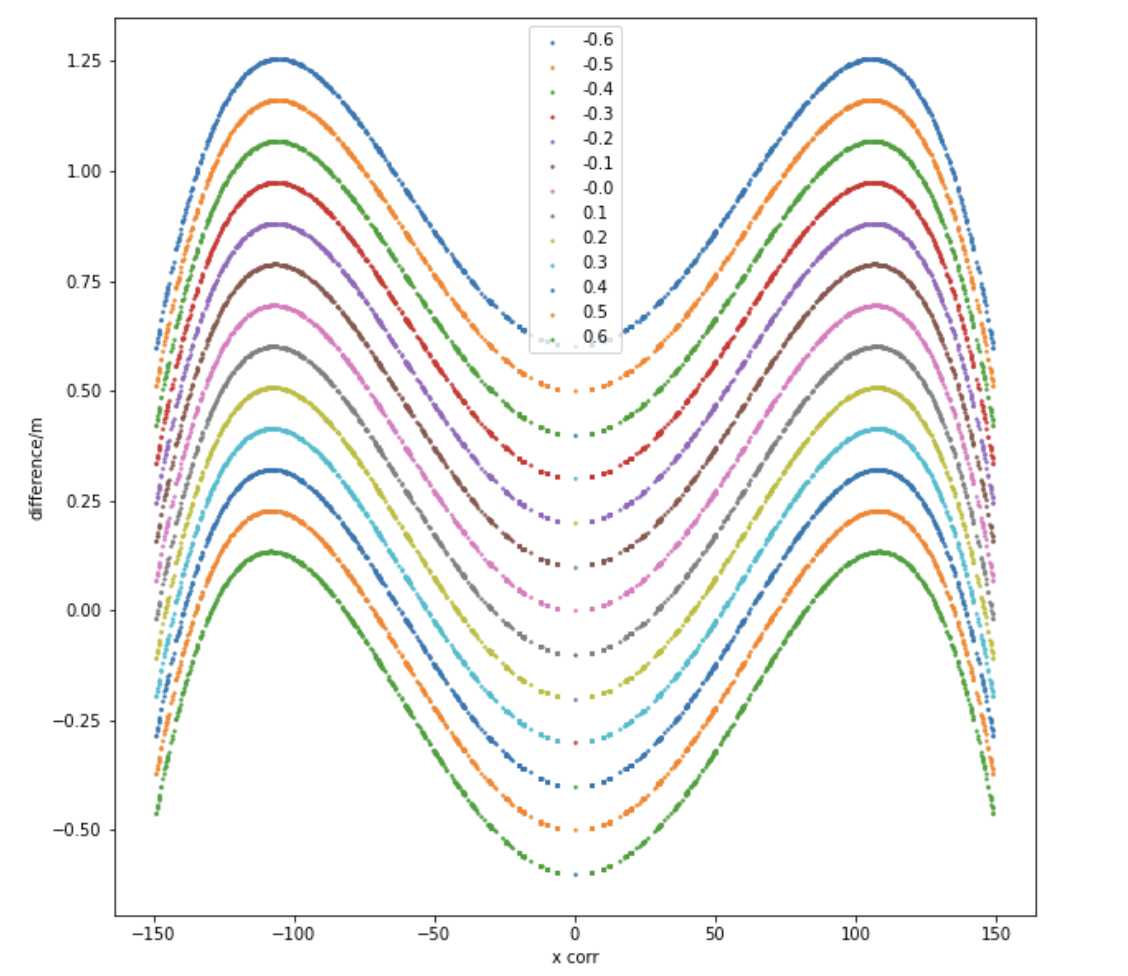
\includegraphics[scale=0.3]{images/cu.png}
    \caption{粗搜索结果图,h分别取-0.6,-0.5..0.6}
\end{figure}



\textbf{$step2$}:在该范围内进行细搜索。

    从上文可以看出,误差曲线的形状大致由焦径比确定,而h决定的是曲线平移量,
可以看出,存在一个最佳h使平移后的误差曲线误差方和最小,从结果可以看出最佳h应该存在于0.3至0.5m,
在这个范围内以0.01m的步长进行搜索得到最小误差的h.

\hspace*{\fill}

\textbf{搜索结果:}

使用变步长搜索得到的最优h为0.397m, 得到最低误差为70.189m,平均到每个主索节点开方后就是0.243m的径向位移,
该值距离0.6m的限制较小,较好的保证了主索节点位移小的要求。

\begin{itemize}
    \item 注意h为距离,非纵坐标,所以调节得到的抛物面顶点低于直线SC与基准球面的交点O。
\end{itemize}

\hspace*{\fill}
\hspace*{\fill}

下图展示了在h=0.397m时,300m口径内不同x坐标的理想抛物线与基准圆的径向差值,该图像为连续光滑的图像表面,相邻主索节点与理想抛物面的差值不会出现
越变,为第二问中的调整方案提供了部分合理性。

\begin{figure}[H]
    \centering
    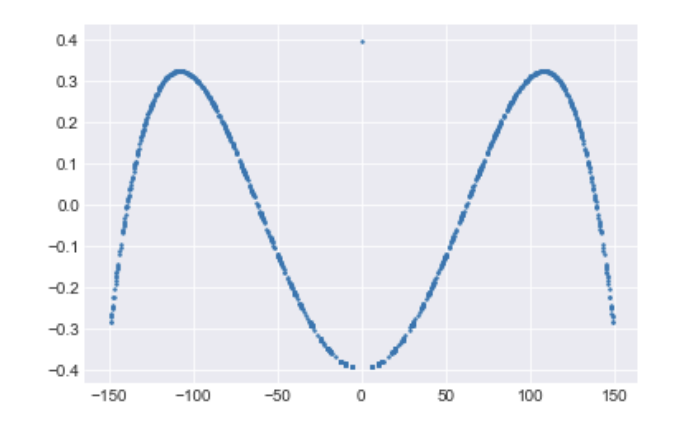
\includegraphics[scale=0.34]{images/xi2.png}
    \caption{主索节点分布图}
\end{figure}


从图中可以看出,径向差值大致均匀分布在0的两侧,做进一步统计有:
所有主索节点中正向位移最大的为0.397m,也就是抛物面顶点,
负向位移最大的为-0.3237m,两值都[-0.6m,0.6m]的范围内,且离边界较远,进一步确保了主索节点伸缩范围的限制条件。


从下直方图可以看出,主索节点的径向距离分布大致均匀,在0.3m处较为集中。

\begin{itemize}
    \item 注:此处的横坐标正方向与题干中促动器伸缩的正方向相反,因此-0.3m就代表促动器伸长0.3m.
\end{itemize}


\begin{figure}[H]
    \centering
    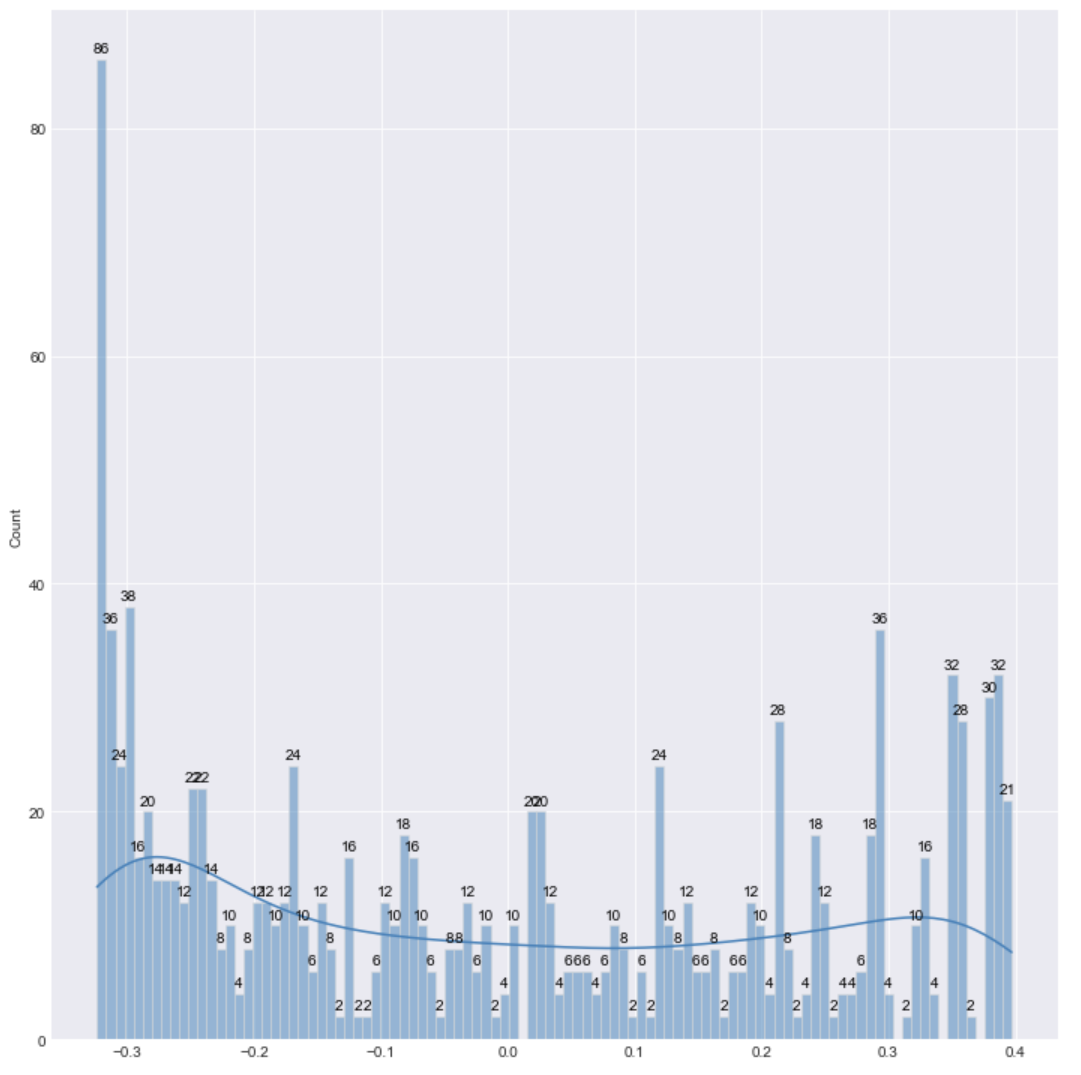
\includegraphics[scale=0.28]{images/xi1.png}
    \caption{主索节点分布直方图}
\end{figure}




综上,我们可以最终得到理想抛物线的方程为:

\begin{equation}
    -x^2+559.2y+167982.0024 =0\quad
\end{equation}

根据题意,将抛物线围绕z轴旋转一周,根据旋转抛物面的对称性,得到\textbf{理想抛物面的方程}为:

\begin{equation}
    -(x^2+y^2)+559.2z+167982.0024 =0\quad
\end{equation}

至此,便完成了问题1的求解。

\vspace{2em}








\subsection{问题2}

\subsubsection{模型准备}
在问题2题干中,我们可以知道S天体位于 $\alpha=36.7956^\circ,\beta=78.169^\circ$ 位置,
由题干中可知SCP位于同一直线上,设理想抛物面的顶点为O,则O在SCP延长线与基准球面交点上。在原有的直角坐标系
中,我们可以利用球面的特性,求出交点O的具体坐标。

设O点坐标为$(x_0,y_0,z_0)$,分析坐标系:

\begin{figure}[H]
    \centering
    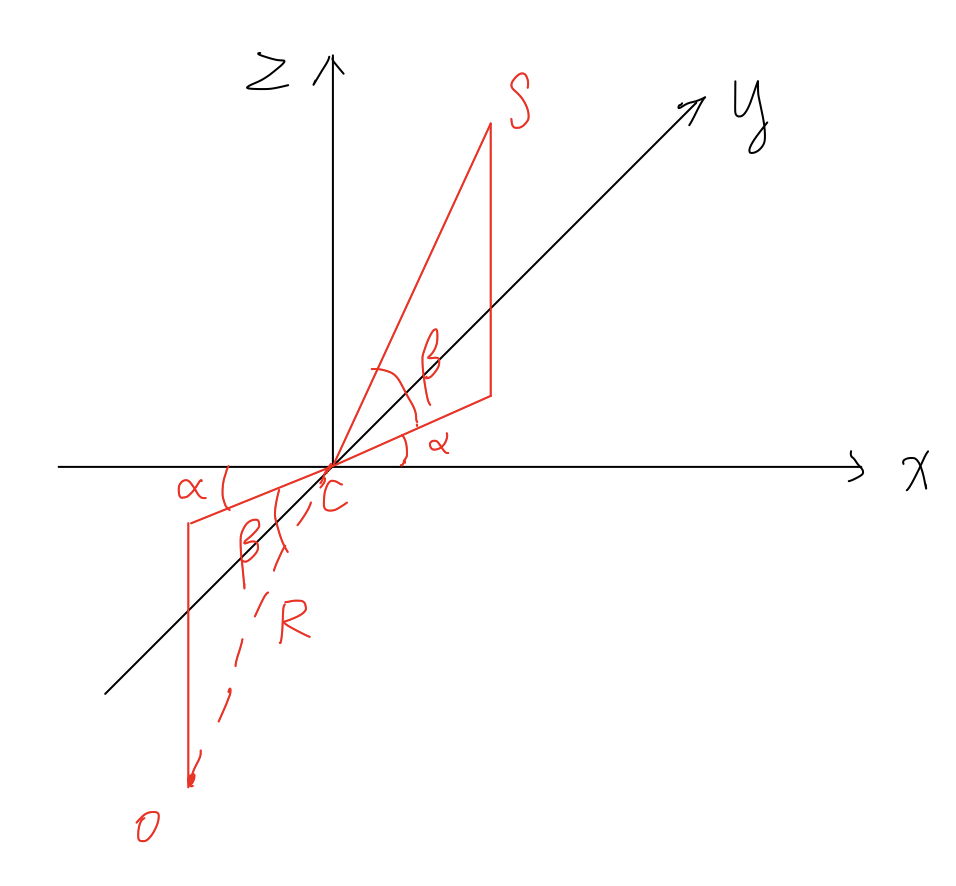
\includegraphics[scale=0.3]{images/zuobiao2.png}
    \caption{天体位置示意图}
\end{figure}


则可以求得O点坐标
\begin{subequations}  
    \begin{numcases}{} 
        x_0 =-Rcos\beta cos\alpha =-49.2539\\ 
        y_0 = -Rcos \beta sin\alpha=-36.8407\\ 
        z_0 = -Rsin\beta=-293.6269
    \end{numcases} 
\end{subequations}

和问题1一样,将问题2转换成二维问题。但由于天体的方位产生了变化,所转化得到的二维平面就会产生一定的倾斜,
就考虑到300m口径的抛物面是否会超出500m口径的问题,示意图如下:
\begin{figure}[H]
    \centering
    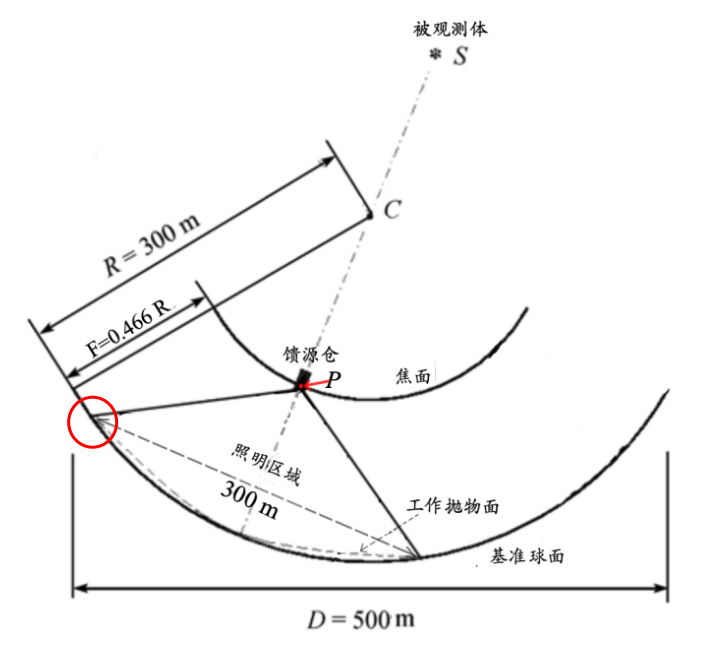
\includegraphics[scale=0.25]{images/pomian.png}
    \caption{二维平面(1)}
\end{figure}

由于围绕直线SC旋转的二维平面有无数个。但由于基准球面是一个各向同性的结构,具有很强的对称性,因此我们只需要分析
过直线SC且平分整个基准球面的这样一个二维平面(红圈处距离基准球碗的高度最小),就能够验证300m口径的理想抛物面是否会超出500m口径的问题。


做出左侧临界情况如下:

\begin{figure}[H]
    \centering
    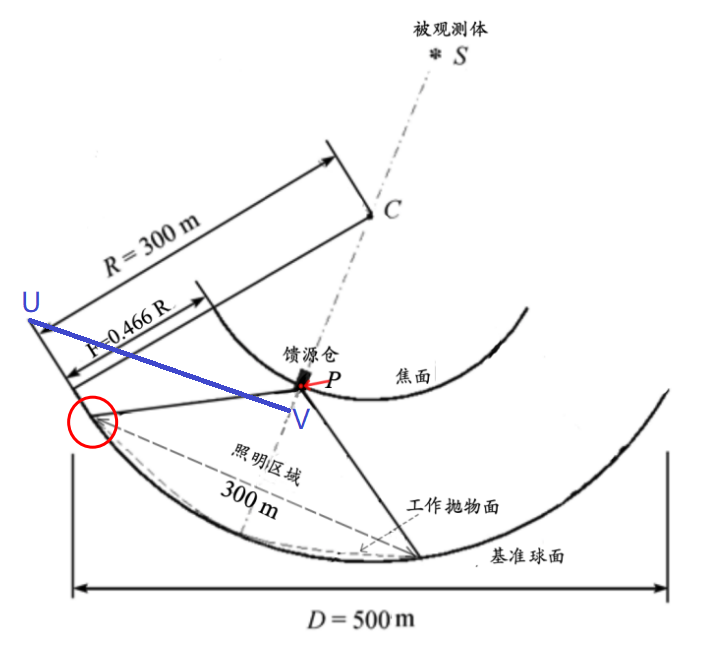
\includegraphics[scale=0.50]{images/pomian3.png}
    \caption{左侧临界情况}
\end{figure}

U为射电望远镜最左端
经过计算得到UV之间的距离为227.73m,该值大于150m,
即口径三百米的抛物面最左侧不会超过射电望远镜的最大限度。
不会产生超出口径的问题。






\subsubsection{第1部分模型建立与求解}
由于基准球面是一个各向同性的结构,以z轴为轴不管怎么旋转都不会改变其基准球面的构造,
所以$\alpha$其实对问题的讨论并没有影响。为了简单起见,不妨设$\alpha = 0^\circ$和问题一的处理方法一样,取$XCZ$平面来研究,
为了方便计算这里记为$X'CY'$。



为了方便处理,我们逆时针旋转坐标系$\gamma = 90^\circ-\beta$得到$X''CY''$平面如下图所示:

\begin{figure}[H]
    \centering
    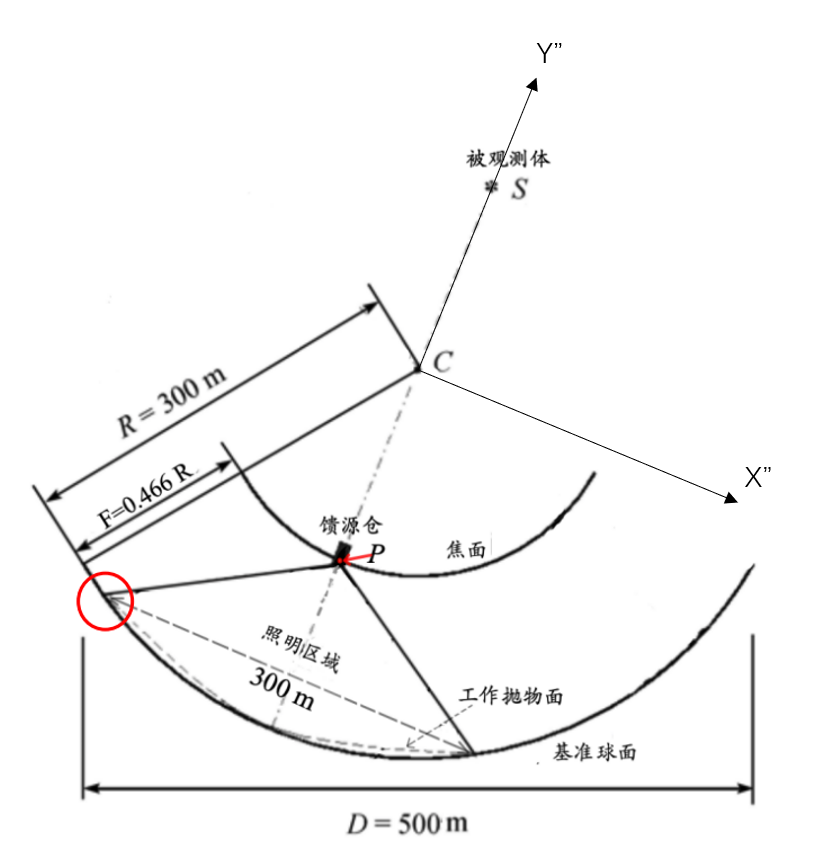
\includegraphics[scale=0.25]{images/pomian2.png}
    \caption{二维平面(2)}
\end{figure}




不妨设原坐标系中的坐标为$(x,y)$,旋转坐标系中旋转后的坐标为$(x^\prime,y^\prime)$

将原有坐标乘以旋转矩阵
$$
\begin{bmatrix}
    cos\gamma& -sin\gamma\\
    sin\gamma& cos\gamma\\
\end{bmatrix}$$

则得到旋转坐标为:
\begin{subequations}  
    \begin{numcases}{} 
        x^\prime =xcos\gamma-ysin\gamma\\
        y^\prime = xsin\gamma+ycos\gamma
    \end{numcases} 
\end{subequations}


同问题1,可以设圆方程和抛物线方程如下:
\begin{subequations}  
    \begin{numcases}{} 
        {x^\prime}^2+{y^\prime}^2=R^2\quad  \\ 
        -{x^\prime}^2+4Dfy^\prime+4Df(R+h) =0\quad
    \end{numcases} 
\end{subequations}

同样的,通过数值求解得到抛物线的数值极坐标方程为:
\begin{equation}
    \rho(\theta,h) = 0.2(37.389838191679836\sqrt{2199+5h+801cos 2\theta+5hcos2\theta}sec^2\theta+1398sec\theta tan\theta)
\end{equation}
   

经过坐标去重和坐标旋转变化后得到x坐标记为$x_i$,记 $ -\arccos( \frac{x_i}{R})$ 为 $\theta_i$

则得到规划模型为:

\begin{equation*}
    Min \sum \quad  (\rho(\theta_i,h)-R)^2
\end{equation*}

\begin{subequations}  
    \begin{numcases}{\text{$s.t$}} 
        -0.6\leq  \rho(\theta_i,h)-R \leq0.6,\quad  \forall i    \\ 
        -0.6\leq h\leq 0.6
    \end{numcases} 
\end{subequations}

经过同问题1相同的求解算法,得到h最优值为0.377m

则理想抛物线在旋转坐标系中的方程为
\begin{equation*}
    -{x^\prime}^2+559.2y^\prime+167970.8184 =0\quad
\end{equation*}

先变为题目所述坐标系,将y还原成字母z,得到方程:
\begin{equation*}
    -{x^\prime}^2+559.2z^\prime+167970.8184 =0\quad
\end{equation*}

然后对其绕对称轴SC进行旋转,在旋转坐标系中z'的坐标不变,且点到对称轴的距离不变,所以令
\begin{subequations}  
    \begin{numcases}{\text{$s.t$}} 
        z = z^\prime \\
        x^\prime = ±\sqrt{x^2+y^2}
    \end{numcases} 
\end{subequations}


\hspace*{\fill}


由此得到旋转坐标系中的抛物面方程为:
\begin{equation}
    -(x'^2+y'^2)+559.2z'+167970.8184 =0\quad
\end{equation}

此时只需要考虑将该方程变换到原有直角坐标系中即可,分为两步骤:

1 绕x轴反转$\gamma$角度

2 绕z轴反转 $90^\circ-\alpha$,记为$\psi$

查阅资料得知,旋转矩阵一般用$4\times 4$的方阵来表示,
但是这里我们这里是绕坐标轴旋转,为了简便起见,采$3\times 3$的
矩阵来表示

两部对应的旋转矩阵分别为:
\begin{math}
\begin{gathered}
    R_1=
    \begin{bmatrix}
        1 & 0 & 0\\
        0 & cos\gamma & -sin\gamma\\
        0 & sin\gamma & cos\gamma\\
    \end{bmatrix}
    \quad
    R_2=
    \begin{bmatrix}
        cos\psi & -sin\psi & 0\\
        sin\psi & cos\psi & 0\\
        0 & 0 & 1\\
    \end{bmatrix}
\end{gathered}
\end{math}

将两种矩阵相乘得到旋转后的坐标为:
\begin{subequations}  
    \begin{numcases}{} 
    x = cos\psi x'-sin\psi cos\gamma y'+sin\psi sin\gamma z'\\
    y = sin\psi x'  + cos\psi cos\gamma y' -sin\psi sin\gamma z'\\
    z = sin\gamma y' + cos \gamma z' 
    \end{numcases} 
\end{subequations}


经过数值求解软件mathematics求得\textbf{最后的理想旋转抛物面}方程为:

\begin{subequations}
    \begin{align}
        &167971 - 0.973045 x^2 - 0.984919 y^2 + y (68.671 + 0.240387 z) \\
        &+ x (91.8091 + 0.0403239 y + 0.321384 z)+ 547.321 z - 0.0420355 z^2 = 0
    \end{align}
\end{subequations}


\subsubsection{结果验证}

经过坐标轴旋转后理想抛物面顶点的坐标:

$$\begin{cases}
x_0 = -49.31586369871079 \\
y_0 = -36.8870732693396 \\
z_0 = -293.9959719830742
\end{cases}$$

对应的入射方向SCP与基准球面的交点:

$$\begin{cases}
x_0 = -49.253967879076114 \\
y_0 =  -36.840776693295034 \\
z_0 =  -293.6269807439393
\end{cases}$$

从理论上分析,这两点相差距离即为h,为前文中搜索得到的h,计算验证确实如此。
证明了坐标变换,旋转过程的正确性。


后文中区分这两个坐标,记理想抛物面顶点坐标为$O$,
记入射方向SCP与基准球面的交点为$O^\prime$.

\hspace*{\fill}

\hspace*{\fill}

\subsubsection{第2部分模型建立与求解}

问题2的第二部分则需要考虑实际调节促动器伸缩,使得主索节点的坐标改变,从而改变反射面板的角度,使之尽可能贴近上述所求的
理想抛物面,为此我们采用基于贪心算法的反射面板调节模型来进行实际调节,基于对问题2的题干的考量:尽可能让
调整后得到的工作抛物面贴近理想抛物面,我们构建调整模型1, 基于对文章需要:以获得天体电磁波经反射后
得到的最佳接受效果作为考量,构建模型2。

\textbf{模型建立}

由于每个主索节点都有6个临近的主索节点(未考虑边界情况,因为调节范围内不涉及边界节点,大部分都是6个
这里假设是6个来分析,少于4个也不影响算法过程),不妨以所有需要考虑的节点V作为节点以节点
间的主索作为边E,以两主索节点的距离作为权重W构建赋权无向图G(V,E,W)。

建立步骤如下:

1:首先找到距离$O^\prime$最近的主索节点记为$V_s$。

2:对于任意一个节点$V_i$的调节:连接$CV_i$交理想抛物面交与$Intersect_i$,
记$Intersect_i$和$V_i$之间的原始距离为$l_i $,$l_i$为从$V_i$到$Intersect_i$的距离,(指向球心为正,否则为负),
需要调节的距离为$d_i$(带符号,符号同题干要求:伸缩沿基准球面径向趋向球心方向为正向)。

具体如下图:

\begin{figure}[H]
    \centering
    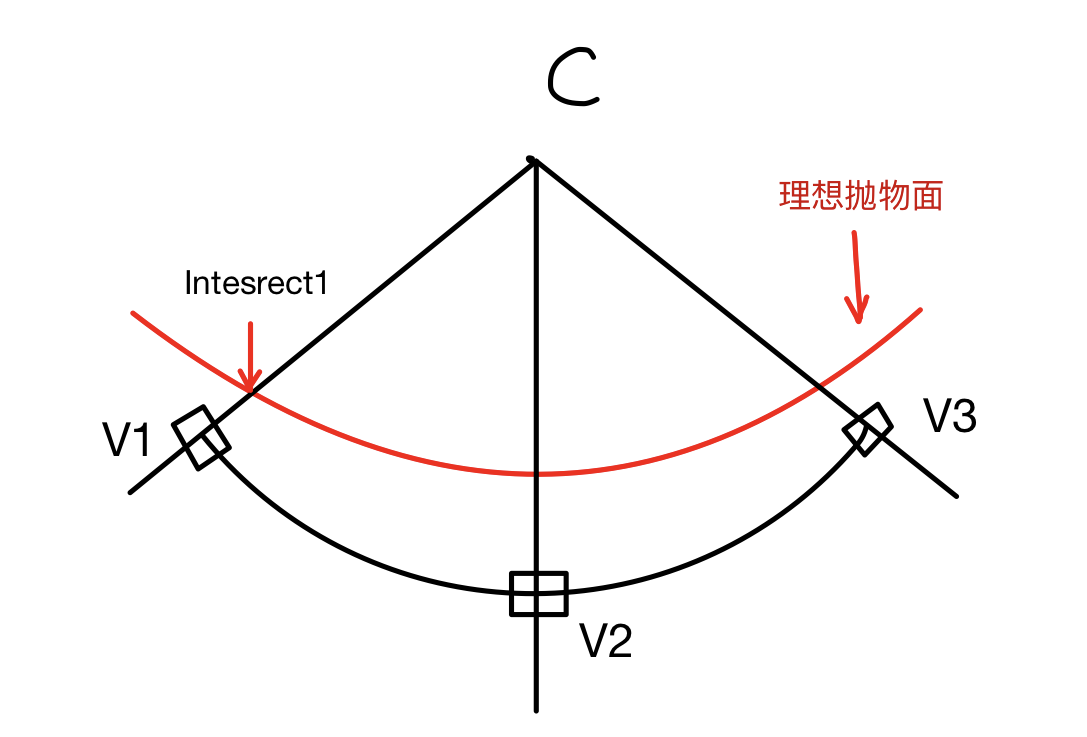
\includegraphics[scale=0.3]{images/wuxiangtu.png}
    \caption{天体位置示意图}
\end{figure}




考虑与$V_i$点相邻的6个主索节点的权重列表$W_i$,记第j个相邻节点与$V_j$的权重为$W_{ij}$。
对于附录要求5中“主索节点调节后,相邻节点之间的距离可能会发生微小变化,变化幅度不超过 0.07\%”
的情况,我们设定该变化幅度为$\sigma $,并假设$\sigma $服从[-0.07\%,0.07\%]的均匀分布,该变化幅度较小,
所以在调整算法中先不予考虑,搜索到最优调整方案后再来讨论该变化幅度的影响。
因而主索节点临近的6个节点的距离(权重) 调整为 $W_{ij}(1+\sigma)$ 。


记$V_i$的坐标为$(x_{v_i},y_{v_i},z_{v_i})$, 则$CV_i$直线方程为:
  $$\frac{x}{x_{v_i}} = \frac{y}{y_{v_i}}=\frac{z}{z_{v_i}}$$

  则联立直线方程和理想抛物面方程:
  $$\begin{cases}
  \frac{x}{x_{v_i}} = \frac{y}{y_{v_i}}=\frac{z}{z_{v_i}}\\
  167971 - 0.973045 x^2 - 0.984919 y^2 + y (68.671 + 0.240387 z) \\
  + x (91.8091 + 0.0403239 y + 0.321384 z) + 547.321 z - 0.0420355 z^2=0\\
  \end{cases}$$


  求得$Intersect_i$的坐标记为$(x_{Intersect_i},y_{Intersect_i},z_{Intersect_i})$
  
  分别计算两点到圆心的距离,记为$d_{CV_i}$和$d_{CIntersect_i}$
  
  则由上定义可得$l_i=d_{CV_i}-d_{CIntersect_i}$

由此得到优化模型:

\begin{equation*}
    Min \quad (l_i-d_i)^2
\end{equation*}

\begin{equation}
    |d_i|\leq 0.6
\end{equation}
        
\hspace*{\fill}

\hspace*{\fill}



\textbf{模型的求解算法}

其求解过程如下:

\begin{itemize}
    \item Step1: 首先找到距离$O'$最近的主索节点记为$V_s$。
    \item Step2: 找到该主索节点的所有临近节点,计算每个节点对应坐标字典,连接$CV_i$交理想抛物面交与$Intersect_i$,计算无向图相关参数。
    \item Step3: 记所有需要调节的节点集合为S,从$V_s$开始调节,然后遍历其相邻的主索节点,进行调节,每调节完一个主索节点后就从S中删去该节点。
    \item Step4: 对于上面调节完的临近主索节点的临近主索节点进行调节,重复操作直至某个需要调节主索节点在S外,此时,判断S是否为空,如果S为空则停止
    调节,调节结束,若S非空,则继续临近主索节点的遍历,直至出现还在S中的节点,继续调整,直至S为空,调整结束。
\end{itemize}

在Step3和Step4中都需要进行调节,调节算法如下:
\begin{itemize}
    \item 1:
    记$V_i$的坐标为$(x_{v_i},y_{v_i},z_{v_i})$, 则$CV_i$直线方程为:
    $$\frac{x}{x_{v_i}} = \frac{y}{y_{v_i}}=\frac{z}{z_{v_i}}$$
    则联立直线方程和理想抛物面方程:
    $$\begin{cases}
        \frac{x}{x_{v_i}} = \frac{y}{y_{v_i}}=\frac{z}{z_{v_i}}\\
        167971 - 0.973045 x^2 - 0.984919 y^2 + y (68.671 + 0.240387 z) \\
        + x (91.8091 + 0.0403239 y + 0.321384 z) + 547.321 z - 0.0420355 z^2=0\\
    \end{cases}$$
    求得$Intersect_i$的坐标记为$(x_{Intersect_i},y_{Intersect_i},z_{Intersect_i})$
    
   \item 2: 分别计算两点到圆心的距离,记为$d_{CV_i}$和$d_{CIntersect_i}$
    
   \item 3: 则由上定义可得$l_i=d_{CV_i}-d_{CIntersect_i}$

   \item 4: 记$V_i$的调整范围的上下界分别为:
   记$d_{MaxAdjustUp_i} = 0.6,d_{MaxAdjustLower_i} =  -0.6 $\
   \item 5: 
   在调整时,采用贪心算法的思路,每一步调整尽可能让目标函数取值最小,分别分四种情况讨论如下:

   (1) $li\geq 0$
   
   
   当 $li\leq d_{MaxAdjustUp_i} $时:
   
   $d_i=l_i$
   
   当 $li > d_{MaxAdjustUp_i} $时:
   
   $d_i=d_{MaxAdjustUp_i}$
   
   
   
   (2) $ l_i< 0$
   
   当$li\geq d_{MaxAdjustLower_i} $时:
   
   $d_i=l_i$
   
   当 $li < d_{MaxAdjustLower_i}$时:
   
   $d_i=d_{MaxAdjustLower_i}$
   
   \item 6: 这样便得到了调整距离,
   每一次调整该节点后就需要修改该节点的坐标,进行保存,然后该节点的调整坐标就确定了,调节过程如下:

 通过直角坐标转化为球坐标方程: $\begin{cases}\rho = \sqrt{x^2+y^2+z^2} \\ \theta = arctan(\frac{\sqrt{x^2+y^2}}{z})\\ \phi = arctan(\frac{y}{x}) \end{cases}$

求得$(x_{v_i},y_{v_i},z_{v_i})$对应的极坐标$(\rho_{v_i},\theta_{v_i},\phi_{v_i})$,然后令$\rho_{v_i}^\prime =\rho_{v_i}-d_i$,
得到调整后的极坐标$(\rho_{v_i}^\prime,\theta_{v_i},\phi_{v_i})$ 

 通过极坐标转直角坐标方程: $\begin{cases}
x = \rho sin\theta cos\phi \\
y = \rho sin\theta sin\phi\\
z = \rho cos\theta
\end{cases}$

基于$d_i$调整极坐标的$\rho$ 回代,便可以得到调整后的直角坐标。
\end{itemize}






  
\textbf{模型的优化} 


文献中指出$^{[3]}$,用球面拟合抛物面的过程实际上是一个用各向曲率均匀的球面去
沿着母线方向曲率各不相同的抛物面,并非将主索节点调控到理想抛物面时拟合精度最优,
而是将其角点偏离抛物面一定距离$d_x$时拟合精度最高,$d_x$是一个基于曲率的值,曲率越大
$d_x$越大.

文献中使用的反射面板为球面,本论文中为了简化计算将其替代为平面,但是性质还是相同的,
平面曲率为定值。 

基于该文献的考量,修改原规划目标函数为:




\begin{equation*}
    Min \quad (l_i-d_x-d_i)^2 \quad \forall i
\end{equation*}

\begin{equation}
    |d_i|\leq 0.6
\end{equation}
        

对于理想抛物面上一点的曲率,这里使用平均曲率带表征,
平均曲率是空间上曲面上某一点任意两个相互垂直的正交曲率的平均值。如果一组相互垂直的正交曲率可表示为K1,K2,那么平均曲率则为:
$H = \frac{K1 +K2 }{2}=\frac{EN-2FM+GL}{2(EG-G^2)}$,其中E,F,G为曲面第一基本系数,L,M,N为曲面第二基本系数.


考虑到解析求解曲率存在困难性,这里依然采用数值求解的方法,
对于每个球心与主索节点连线交理想抛物面的点,设该点为$(x,y,z)$,则在$[x-0.1,x+0.1)$范围内取5个点,则在$[y-0.1,y+0.1)$范围内取5个点,meshgride后得到25个点,然后用这25个点计算其对应的平均斜率$H_j,\quad j =1,2...25$ ,
平均斜率的计算方法采用曲面拟合的思想,用一阶导数和二阶导数以及曲面第一第二基本系数,计算得到(具体代码见“代码”文件夹), 则用$\sum H_j$作为该点处的平均斜率。



   关于$d_x$和$H$的关系,我们不妨假设其存在一次函数和二次函数的关系,分别为
   $d_x =k_1H,d_x=k_2H^2$, 分别考虑一次函数和二次函数的方案进行参数搜索。

   
综上,最终的反射面板调节的数学模型如下:

$$
    Min \quad (l_i-d_x-d_i)^2 \quad \forall i
$$ 

\begin{subequations}  
    \begin{numcases}{$s.t$} 
        \mbox{其中} dx = k_1H \mbox{或} dx=k_2H^2,\\
        H=\sum_{j=1}^{25} H_j,H_j = \frac{EN-2FM+GL}{2(EG-G^2)} \\
        |d_i|\leq 0.6
    \end{numcases} 
\end{subequations}



\hspace*{\fill}

考虑到第三问的需求需要我们计算馈源舱接受比率,那么不妨以馈源舱接受率作为限制条件来
搜索k以及模型,接受率的求解方法在第三问中,下面基于$dx=kH^2$的形式构建规划模型,
$dx = k_1H $时同理。

\begin{equation*}
    Min \quad  \omega
\end{equation*}

$$\begin{cases}
        Min \quad (l_i-d_x-d_i)^2 \quad \forall i \\ 
          \mbox{其中}  dx=k_2H^2,\\
           H=\sum_{j=1}^{25} H_j ,H_j = \frac{EN-2FM+GL}{2(EG-G^2)} \\
           |d_i|\leq 0.6 \\
    \end{cases}$$


    \hspace*{\fill}

    \hspace*{\fill}

    \textbf{ 优化后的模型的求解以及结果}


    

  依然采用问题1中使用的变步长搜索对其进行搜索,搜索得到的结果为$k=27.25,\omega = 65.8\%$, 
  关于接受率的详细讨论在第三问。 下面对搜索得到的调整方案做说明(对于$dx = k_1H $的情况也做了搜索,发现其馈源舱接受率都普遍低于$dx=kH^2$
  的形式,所有后文中没有予以讨论。):

  通过计算,所有主索节点中,在该口径范围内的节点有720个,下图展示了这720个主索节点
  对应的促动器上端点调整距离. 

  \begin{figure}[H]
    \centering
    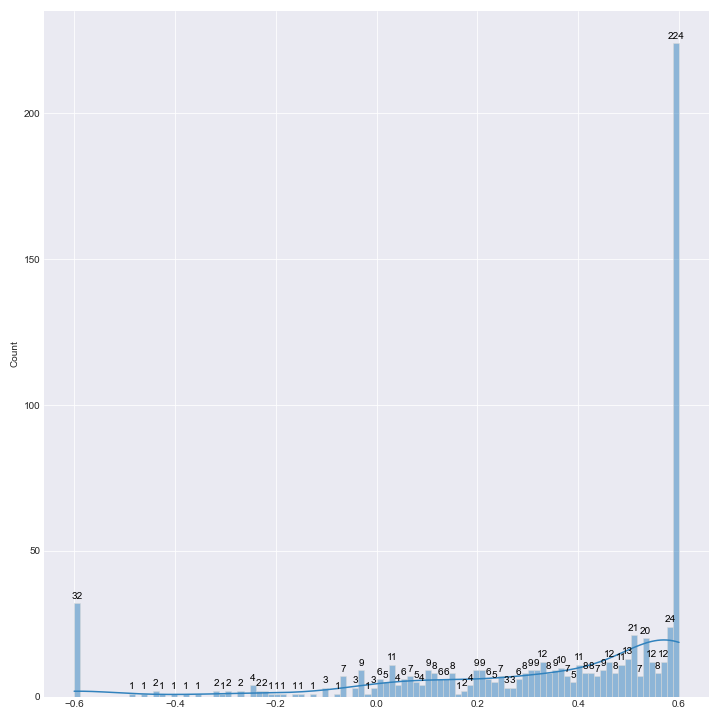
\includegraphics[scale=0.3]{images/sta2r.png}
    \caption{促动器调节距离}
\end{figure}

可以看出大多数主索节点的调节距离在$[0,0.6]$附近,0.6处较为集中,大概占据了所有调节点数量的
$\frac{1}{3}$,在-0.6处也存在较多,大概占5\%,可以看出,该调节方案
对主索节点的调节还是较大的。在第三问将根据接受比来判断调整方案的效果。

\hspace*{\fill}

\hspace*{\fill}

\hspace*{\fill}


\textbf{ $\sigma$ 对调整方案的影响} 


考虑到两临近主索节点的距离大概为10m左右,基于一个上下0.07\%的波动就是[9.993,10.007] ,由于上下界的波动是一样的而且波动远小于R(300m),可以认为
其对主索节点径向方向的影响上下界是范围是相同的,不难求出其波动范围为[-0.16648,+0.16648] 对应到主索节点的,考虑到工程中,波动发生的概率较小,不妨
设该主索节点有P的可能性不发生波动,只有1-P的可能性会发生波动.

假设P = 80\% ,考虑该情况下对主索节点调整距离加上该波动可以得到该调整方案下不同节点的波动如下:

\begin{figure}[H]
    \centering
    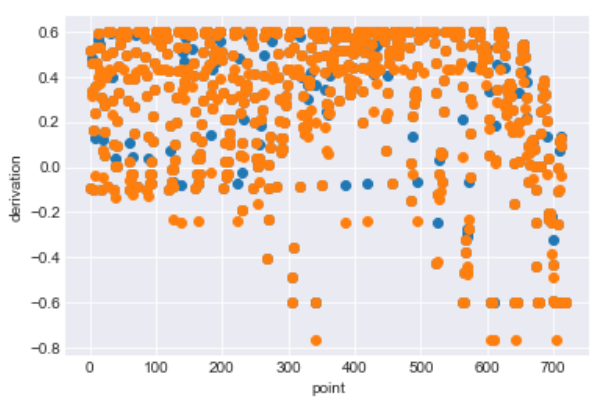
\includegraphics[scale=0.3]{images/bodong.png}
    \caption{调整距离的波动}
\end{figure}

可以看到,部分主索节点的调整距离会发生改变,可以预见的是P值越大,这些会发生波动的主索节点越少,而对于波动区间,相比于最大调整幅度为0.6m ,0.16648
已经算是一个比较大的波动了,考虑到发生波动可能性的存在,如果可能性大的话,将会对调整方案产生较大影响,如果较小的话,则对调解方案的影响可以忽略。  

\hspace*{\fill}

\hspace*{\fill}
\subsection{问题3}

\subsubsection{问题3模型的建立}

在问题2中已经设计好反射面的调节方案,为了衡量反射面的调节后的实际效果,需要计算出馈源舱的接受比并与基准反射球面的接受比进行比较。
在问题1与问题2中都将整个反射面作为一个整体抛物面进行建模分析,在本问题中则需要进行局部分析,即对每一块反射板的情况进行分析,
计算出相应的入射信号与反射信号的轨迹,从而定量确定倍馈源舱接收到的有效反射信号。


\subsubsection{反射面板对信号的反射}

由于信号发射源S与观测点的距离极大,所以入射电磁波可以视作平行信号,方向向量为CP,在不同位置的反射面板上反射汇聚,
部分信号汇聚与P点被馈源舱接收。

\begin{figure}[H]
    \centering
    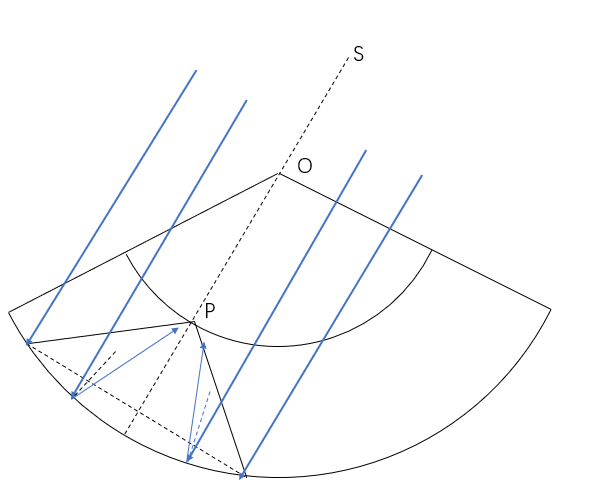
\includegraphics[scale=0.3]{images/fanshe.png}
    \caption{光线反射图}
\end{figure}


由于整个反射面是由许多块反射面板拼接而成,每块面板位置不同从而反射情况也不同,因此需要对每一块反射板的反射情况进行分析。


\begin{figure}[H]
    \centering
    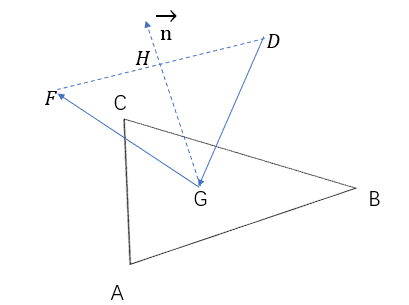
\includegraphics[scale=0.3]{images/ban.png}
    \caption{反射面板示意图}
\end{figure}

由上图所示,反射面板具有三角形结构,由于相邻节点间的距离大约在10米左右,较曲率半径300米较小,因此将反射面板
近似为平面分析,相邻三个主索节点坐标可作为其顶点坐标,为了方便讨论,只考虑入射信号在三角形重心G的反射情况。G的坐标:

\begin{equation}
    P_G=\frac{P_A+P_B+P_C}{3}
\end{equation}

已知天体方位角α与方位角β,入射信号的方向向量:
\begin{equation}
    \overrightarrow {n_1} = -(cos\beta cos\alpha , cos\beta sin\alpha, sin\beta)
\end{equation}

任取入射信号上异于G一点D,则:
\begin{equation}
    \overrightarrow{OP_D} = \overrightarrow{OP_G} - \overrightarrow{n_1}
    \label{H}
\end{equation}

因而平面ABC的法向量为:
\begin{equation}
    \overrightarrow{n} = \overrightarrow{P_AP_C} \times \overrightarrow{P_AP_B}
    \label{n}
\end{equation}

根据反射定理,入射信号,反射信号与法线$\overrightarrow{n}$均在同一平面内,H为垂足,则GH与$\overrightarrow{n}$之比为:

\begin{equation}
    t_1=\frac{|\overrightarrow{n}\cdot \overrightarrow{P_DP_G}|}{|\overrightarrow{n} \cdot \overrightarrow{n}|}
    \label{t}
\end{equation}

可得到垂足H点坐标为:
\begin{equation}
    \overrightarrow{OP_H}=\overrightarrow{OP_G}+t_1 \cdot \overrightarrow{n}
    \label{H}
\end{equation}

H点为FD的中点,可以求出F点坐标$P_F$与反射信号的方向向量$\overrightarrow{n_2}$
\begin{align}
    \overrightarrow{OP_F} &= 2\overrightarrow{OP_H} - \overrightarrow{OP_D}\\
    \overrightarrow{n_2} &= \overrightarrow{P_GP_F}
\end{align}

确定好反射信号方向向量与经过点G可以计算出与馈源舱所在平面的交点Q的坐标$P_Q$,
并判断是否落在馈源舱平面内,P点为馈源舱位置,第i块面板反射信号落在馈源舱情况定义为$a_i$:

\begin{subequations}
    \begin{numcases}{}
        1,|\overrightarrow{P_QP_P}|\leq0.5\\
        0,|\overrightarrow{P_QP_P}|> 0.5
    \end{numcases}
\end{subequations}

易求得第i块面板的重心与直线OP的距离为$D_i$,则第i块面板反射信号落在照明区域情况定义为$b_i$:

\begin{subequations}
    \begin{numcases}{}
        1,D_i\leq150\\
        0,D_i > 150
    \end{numcases}
\end{subequations}

 \subsubsection{反射面板有效反射面积}


假定接收信号是空间内均匀分布的,则落在反射板上的有效面积为反射板在以入射方向为法向量所在平面内的投影面积。


\begin{figure}[H]
    \centering
    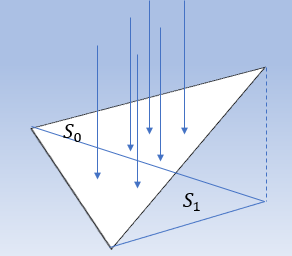
\includegraphics[scale=0.3]{images/touying1.png}
    \caption{投影示意图}
\end{figure}



任取投影平面$Ax+By+Cz+D=0$,,则三维空间坐标点$(x_0,y_0,z_0)$在投影平面上的投影点坐标为:


$$x_p=\frac{(B^2+C^2)x_0-A(By_0+Cz_0+D)}{A^2+B^2+C^2}$$

$$y_p=\frac{(A^2+C^2)x_0-B(AX_0+Cz_0+D)}{A^2+B^2+C^2}$$

$$z_p=\frac{(A^2+B^2)z_0-C(Ax_0+By_0+D)}{A^2+B^2+C^2}$$

可根据公式计算获得反射板顶点坐标的投影点J K L,则第i块反射面板投影面积
$S_i$为:

\begin{equation}
    S_i=\frac{|\overrightarrow{JK}\times \overrightarrow{KL}|}{2}
\end{equation}


将所有处于照明区域且反射光线汇聚与馈源舱有效区域的反射面板投影面积累加,然后除以总入射信号面积,则\textbf{接收比}$\omega$为:

\begin{equation}
    \omega = \frac{\sum_{i=1}^{4300}Si*a_i*b_i}{150^2\pi}
\end{equation}


\subsubsection{模型求解与结果分析}

附件一中给出了所有主索节点的坐标,即各个反射面顶点坐标,附件三中给出了4300块反射面板的顶点编号,
从而可以求取每个反射面重心坐标,结合入射光线方向向量与反射面的法向量求的反射信号方程,并判断是否汇聚到馈源舱的有效区域,
统计所有的有效反射信号对应反射面板的投影面积之和,
求出基准球面接收比。然后替换修改后的主索节点坐标,求出调整后馈源舱的接受比。

\begin{figure}[H]
    \begin{minipage}[t]{0.5\linewidth}
    \centering
    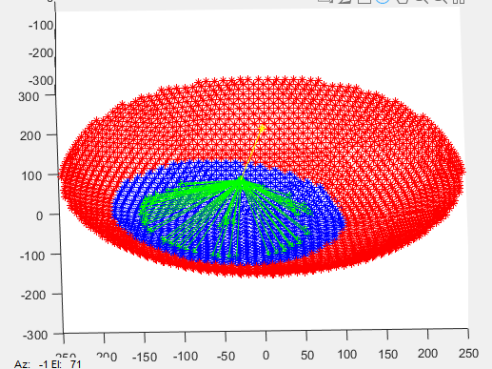
\includegraphics[scale=0.35]{images/jieguo1.png}
    \caption{调整前有效反射信号示意图}
    \label{fig:side:a}
    \end{minipage}%
    \begin{minipage}[t]{0.5\linewidth}
    \centering
    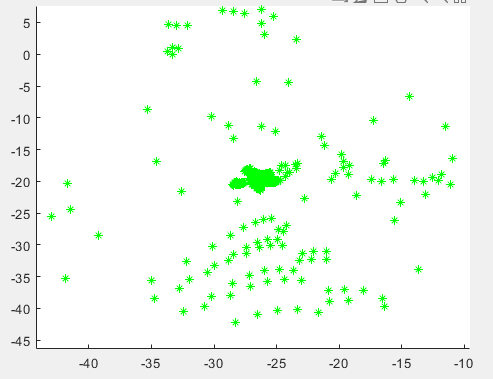
\includegraphics[scale=0.45]{images/xinjieguo1.png}
    \caption{调整前馈源舱所在平面散点图}
    \label{fig:side:b}
    \end{minipage}
\end{figure}

\begin{figure}[H]
    \begin{minipage}[t]{0.5\linewidth}
    \centering
    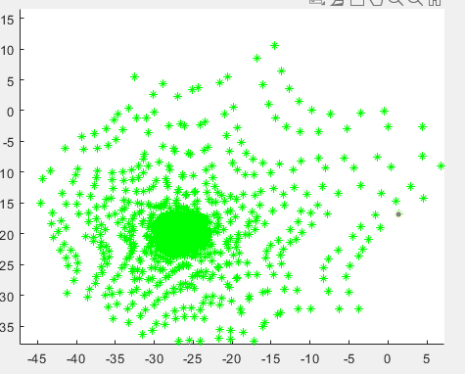
\includegraphics[scale=0.3]{images/jieguo2.png}
    \caption{调整后有效反射信号示意图}
    \label{fig:side:c}
    \end{minipage}%
    \begin{minipage}[t]{0.5\linewidth}
    \centering
    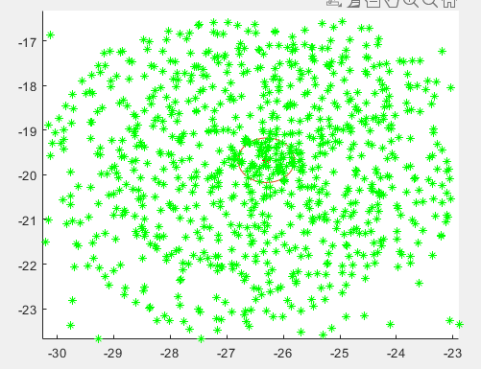
\includegraphics[scale=0.3]{images/jieguo3.png}
    \caption{调整后馈源舱所在平面散点图}
    \label{fig:side:d}
    \end{minipage}
\end{figure}

最终计算出来基准球面接收比$\omega$为11.3\%,经过调整后馈源舱的接收比$\omega$为65.9\%。主动反射面反射情况与馈源舱所在平面反射信号分布情况如上图所示,
蓝色区域为照明区域,绿色线为汇聚到馈源舱的反射光线,黄色线为馈源舱与原点的连线。在未调整前,图四中反射汇聚信号较为稀疏,
分布较为均匀,在经过调整后,图六中反射到馈源舱平面内的信号明显增加。

右侧图为馈源舱所在平面所有反射信号的在馈源舱所在平面的分布情况,可以看到为调整前,
图五中信号较为分散,汇聚于馈源舱的信号较少,在调整后,图七中信号集中于馈源舱所在位置附近。



由上述分析可得到在经过调整后反射到馈源舱的信号大幅度增加,制定的调整方案较为合理,有利于汇聚外来信号进行科学研究,获取更多有用信息。

基于第二问中假设的80\%发生波动的情况,再次计算了该情况下的馈源舱接收比:  30\% , 可以认为,该波动对问题2中的方案调整具有较大影响,会使
馈源舱接收比显著下降,为了达到更好的接受效果,调整过程中应尽量减少波动的发生。


\hspace*{\fill}

\hspace*{\fill}

\hspace*{\fill}

\hspace*{\fill}






\section{模型的评价与推广}

\subsection{模型的优点}

1.模型参考了"FAST"有关的可靠文献,提出了较合理的衡量反射面板与理想抛物面误差的方案。

2.模型将连续问题离散化,进行变步长搜索,先粗调再细调,搜索速度快,巧妙地解决了优化问题。

3.模型将三维问题转化到二维平面进行分析,进行了相当的简化。

\subsection{模型的缺点}

1.模型近似过程较多,对于光线光路可能存在一定影响。

2.模型所得到的结果难以验证。

3.忽略了馈源舱不同部分接受到的光强差异所产生的影响。

\subsection{模型的改进与推广}

\begin{itemize}
\item 可对于每个反射面板以球面反射进行更细致的分析,进一步提高接受比。
\item 可采用遗传算法等搜索出贪心算法中开始调节的起点。
\item 模型本身在"FAST"球面射电望远镜已经大获成功的前提下具有一定的可行性,
在其他球面结构的望远镜中可同样适用,具有普遍意义。
\end{itemize}



\newpage
    \begin{thebibliography}{9}%宽度9
        \bibitem [1] 
        \newblock 朱丽春.
        \newblock 500米口径球面射电望远镜(FAST)主动反射面整网变形控制[J].
        \newblock 科研信息化技术与应用,2012,3(04):71.

        \bibitem [2] 
        \newblock 李明辉,朱丽春.
        \newblock FAST瞬时抛物面变形策略优化分析[J].
        \newblock 贵州大学学报(自然科学版),2012,29(06):25

        \bibitem [3] 
        \newblock 钱宏亮.
        \newblock FAST主动反射面支承结构理论与试验研究[D].
        \newblock 哈尔滨工业大学,2007:2(27).
       


    \end{thebibliography}


\newpage
    \begin{appendices}

        \section{问题1的代码}
        \begin{lstlisting}[language=python]
            import pandas as pd 
import numpy as np
import matplotlib.pyplot as plt
df = pd.read_csv("附件1.csv",encoding="GBK")
df

x = df['X坐标(米)']
y = df['Y坐标(米)']
z = df['Z坐标(米)']


ax = plt.gca(projection='3d')
ax.scatter(x,y,z,s=1)


ax = plt.gca(projection='3d')
ax.view_init(0,0)
ax.scatter(x,y,z,s =1)

len(set(x))


import numpy as np
from scipy import optimize		# 最小二乘法拟合
import matplotlib.pyplot as plt 	# python matplotlib 绘图
from mpl_toolkits.mplot3d import Axes3D  # 3D 绘图


def func(x, y, p):
	""" 数据拟合所用的函数:z=ax+by
	:param x: 自变量 x
	:param y: 自变量 y
	:param p: 拟合参数 a, b
	"""
	a, b = p
	return a+b*(x**2+y**2)


def residuals(p, z, x, y):
	""" 得到数据 z 和拟合函数之间的差
	"""
	return z - func(x, y, p)


def main():
	#x = np.arange(5)
	#y = np.arange(5)
	#z = np.array([2, 4, 7, 7, 10])  # 数据随便取的

	plsq = optimize.leastsq(residuals, np.array([0, 0]), args=(z, x, y))  # 最小二乘法拟合

	a, b = plsq[0]  # 获得拟合结果
	print("拟合结果:\na = {}".format(a))
	print("b = {}".format(b))

	# 绘图
	xp = np.linspace(-300, 300, 100)
	yp = np.linspace(-300, 300, 100)

	X, Y = np.meshgrid(xp, yp)
	Z = func(X, Y, [a, b])   # 带入拟合得到的 a, b
	fig = plt.figure(figsize=(8, 6))
	ax = Axes3D(fig)    # 3D 绘图

	ax.plot_surface(X, Y, Z, alpha=0.5,color="b")
	ax.scatter(x, y, z, color="green",s=1)

	ax.set_xlabel("x")
	ax.set_ylabel("y")
	ax.set_zlabel("z")

	plt.show()


if __name__ == "__main__":
	main()

nx =[]
ny =[]
nz = []
for i in range(len(x)):
    if np.abs(x[i])>=150 or np.abs(y[i])>=150 : 
        pass 
    else :
        nx.append(x[i])
        ny.append(y[i])
        nz.append(z[i])
        

# 第一问求解


## F>$\frac{1}{4b}$时
a=  -306.02002053903254
b = 0.00186
mse = 0
for i in range(len(nx)):
    mse+= (a+b*(nx[i]**2+ny[i]**2)-nz[i])**2
print(mse/len(x))

1/(4*0.00177321397)

 0.00186321397*4*F

1/(4*0.001863)

b = 0.001863
R = 300
F=0.466*R
D =(2-8*b*F+np.sqrt((-2+8*b*F)**2-16*b**2*(-1+4*a*b+4*b*R)))/(8*b**2)
print(D**2*4/R**2)

# 4bF<1 


b =  0.00186321397
R = 300
F=0.466*R
D =(-2+8*b*F+np.sqrt((-2+8*b*F)**2-16*b**2*(-1+4*a*b+4*b*R)))/(8*b**2)
print(D**2*4/R**2)


import numpy as np
from scipy import optimize		# 最小二乘法拟合
import matplotlib.pyplot as plt 	# python matplotlib 绘图
from mpl_toolkits.mplot3d import Axes3D  # 3D 绘图


def func(x, y, p):
	""" 数据拟合所用的函数:z=ax+by
	:param x: 自变量 x
	:param y: 自变量 y
	:param p: 拟合参数 a, b
	"""
	a, b = p
	return a+b*(x**2+y**2)


def residuals(p, z, x, y):
	""" 得到数据 z 和拟合函数之间的差
	"""
	return z - func(x, y, p)


def main():
	x=np.array(nx)
	y=np.array(ny)
	z=np.array(nz)
	#x = np.arange(5)
	#y = np.arange(5)
	#z = np.array([2, 4, 7, 7, 10])  # 数据随便取的
	plsq = optimize.leastsq(residuals, np.array([0, 0]), args=(z, x, y))  # 最小二乘法拟合

	a, b = plsq[0]  # 获得拟合结果
	print("拟合结果:\na = {}".format(a))
	print("b = {}".format(b))

	# 绘图
	xp = np.linspace(-150, 150, 100)
	yp = np.linspace(-150, 150, 100)

	X, Y = np.meshgrid(xp, yp)
	Z = func(X, Y, [a, b])   # 带入拟合得到的 a, b
	fig = plt.figure(figsize=(8, 6))
	ax = Axes3D(fig)    # 3D 绘图

	ax.plot_surface(X, Y, Z, alpha=0.5,color="b")
	ax.scatter(x, y, z, color="green",s=1)

	ax.set_xlabel("x")
	ax.set_ylabel("y")
	ax.set_zlabel("z")

	plt.show()


if __name__ == "__main__":
	main()


x_t = np.arange(-300,300,0.01)
y_1 = -np.sqrt(300**2-x_t**2)
y_3 = +np.sqrt(300**2-x_t**2)
y_2 = -(1.6625e5-x_t**2)/(2*276.6470)
plt.scatter(x_t,y_1,s=0.00001)
plt.scatter(x_t,y_3,s=0.00001)
plt.scatter(x_t,y_2,s=0.00001)



x_testify = np.array(list(set(x))) # 用来检验的x
x_testify = x_testify[np.where(np.abs(x_testify)<=150)]
x_testify.size


def get_delta_R_for_x_i(x_i,h):
    # 获得x_i对应的径向距离差
    D=R=300
    f=0.366
    theta = -np.arccos(x_i/R)
    # 由于x_i接近0时float的误差会导致原式发生较大误差故:
    if np.abs(x_i)<1e-4:
        return h 
    rho = 0.2*(37.389838191679836*np.sqrt(2199+5*h+801*np.cos(2*theta)+5*h*np.cos(2*theta))*
    (1/(np.cos(theta)))**2+1398*np.tan(theta)/np.cos(theta))
    result = rho-R
    return result
def get_judge_error(arry):
    return np.sum(np.square(arry)) # 返回拟合标准, 即差值,差值要尽可能小

def satisfy_requirement(arry):
    maximum = np.max(np.abs(arry)) # 最大误差 , 其为取绝对值后的最大误差
    if maximum <=0.6:
        return True # 满足条件
    else :
        return False 
    

hs = np.arange(-0.6,0.7,0.1)
plt.figure(figsize=(10,10))
for  h in hs: # w遍历每个h 
    tempt =x_testify
    tempt_y = []
    for i in tempt:
        tempt_y.append(get_delta_R_for_x_i(i,h))
    if(satisfy_requirement(tempt_y)):
        print("满足要求的h=%.1f"%h,"其对应的误差为:%.2f"%get_judge_error(tempt_y))
    plt.scatter(tempt,tempt_y,s=2)
    plt.xlabel("x corr")
    plt.ylabel("difference/m")
plt.legend(["%.1f"%h for h in hs])


hs = np.arange(0.3,0.5,0.001)
min_error  = float("inf")# 给予初始值
optimal_h = float("inf")
for  h in hs: # w遍历每个h 
    tempt =x_testify
    tempt_y = []
    
    for i in tempt:
        tempt_y.append(get_delta_R_for_x_i(i,h))
    if(satisfy_requirement(tempt_y)):
        if get_judge_error(tempt_y)<min_error:
            min_error = get_judge_error(tempt_y)
            optimal_h = h
        #print("满足要求的h=%.3f"%h,"其对应的误差为:%.2f"%get_judge_error(tempt_y))



import seaborn as sns
import os
# 这里是对画布的设置。num 是 数字或者字符串,是figure的名字。
# subplots是方便多个子图(只有一个图的时候写1,1就行)
fig, axes = plt.subplots(1, 1, num="stars",figsize=(10, 10))#, sharex=True)
# 使用画布背景。
plt.style.use('seaborn-darkgrid') #'seaborn-bright'
# 调色板,可以使用里面的颜色 color,还挺好看的
palette = plt.get_cmap('tab20c')#'Pastel2') # 'Set1' 
plt.subplot(1, 1, 1)
# 调用histplot作图
ax1 = sns.histplot(tempt_y, kde = True, bins = 100, shrink = 1, color = palette.colors[0], edgecolor = palette.colors[-1])#"none")#, element="step")# element = "poly") # cumulative = True)

# ax.invert_yaxis() 
# plt.gca().invert_yaxis()
# newx = ax.lines[0].get_ydata()
# newy = ax.lines[0].get_xdata()

# # set new x- and y- data for the line
# ax.lines[0].set_xdata(newx)
# ax.lines[0].set_ydata(newy)

# plt.subplot(2, 1, 2)
# sns.distplot(df["stars"], kde = True, bins = 20)# element="step", fill=False)

# 给直方图添加文字注释(就是在每一个bar的上方加文字)
for p in ax1.patches:
    if p.get_height() > 0:
        ax1.annotate(
            # 文字内容
            text=f"{p.get_height():1.0f}",
            # 文字的位置
            xy=(p.get_x() + p.get_width() / 2., p.get_height()), 
            xycoords='data',
            ha='center', 
            va='center', 
            fontsize=10, 
            color='black',
            # 文字的偏移量
            xytext=(0,7), 
            textcoords='offset points',
            clip_on=True,                   # <---  important
        )

# 紧密排版
plt.tight_layout()
# 保存图片
plt.savefig("star.png")
plt.show()


tempt_y = []
for i in tempt:
        tempt_y.append(get_delta_R_for_x_i(i,0.3970000000000001))
print(max(tempt_y),min(tempt_y))
plt.scatter(tempt,tempt_y,s=2)
   



        \end{lstlisting}

        \section{问题2的代码}
        \begin{lstlisting}[language=python]
            import numpy as np
            import matplotlib.pyplot as plt
            k_1 = 4.7738
            x = np.arange(-250,250,0.01)
            y_c = -np.sqrt(300**2-x**2)
            for k in np.arange(-2000,2000,100):
                plt.plot(np.arange(-200,200,0.1),k_1*np.arange(-200,200,0.1))
            plt.plot(x,y_c)

            import math
alpha = math.radians(36.7956)
beta = math.radians(78.169)

x=-300*math.cos(beta)*math.cos(alpha)
y= -300*math.cos(beta)*math.sin(alpha)
z = -300*math.sin(beta)
x,y,z

import pandas as pd 
import numpy as np
import matplotlib.pyplot as plt
df = pd.read_csv("附件1.csv",encoding="GBK")
df

x = df['X坐标(米)']
y = df['Y坐标(米)']
z = df['Z坐标(米)']

gamma = math.radians(90)-beta
gamma

x_testify = np.array(x) # 用来检验的x
y_testify = np.array(z)
x_testify_prime = x_testify*np.cos(gamma)-y_testify*np.sin(gamma)
y_testify_prime = x_testify*np.sin(gamma)+y_testify*np.cos(gamma) # 坐标变换

x_testify_prime = np.array(list(set(x_testify_prime))) # 去重
x_testify_prime.size

x_testify_prime = x_testify_prime[np.where(np.abs(x_testify_prime)<=150)]
x_testify_prime.size # 只取300口径内的


def get_delta_R_for_x_i(x_i,h):
    # 获得x_i对应的径向距离差
    D=R=300
    f=0.366
    theta = -np.arccos(x_i/R)
    # 由于x_i接近0时float的误差会导致原式发生较大误差故:
    if np.abs(x_i)<1e-4:
        return h 
    rho = 0.2*(37.389838191679836*np.sqrt(2199+5*h+801*np.cos(2*theta)+5*h*np.cos(2*theta))*
    (1/(np.cos(theta)))**2+1398*np.tan(theta)/np.cos(theta))
    result = rho-R
    return result
def get_judge_error(arry):
    return np.sum(np.square(arry)) # 返回拟合标准, 即差值,差值要尽可能小

def satisfy_requirement(arry):
    maximum = np.max(np.abs(arry)) # 最大误差 , 其为取绝对值后的最大误差
    if maximum <=0.6:
        return True # 满足条件
    else :
        return False 

        hs = np.arange(-0.6,0.7,0.1)
        plt.figure(figsize=(10,10))
        for  h in hs: # w遍历每个h 
            tempt =x_testify_prime
            tempt_y = []
            for i in tempt:
                tempt_y.append(get_delta_R_for_x_i(i,h))
            if(satisfy_requirement(tempt_y)):
                print("满足要求的h=%.1f"%h,"其对应的误差为:%.2f"%get_judge_error(tempt_y))
            plt.scatter(tempt,tempt_y,s=2)
            plt.xlabel("x corr")
            plt.ylabel("difference/m")
        plt.legend(["%.1f"%h for h in hs])

        hs = np.arange(0.3,0.5,0.001)
        min_error  = float("inf")# 给予初始值
        optimal_h = float("inf")
        for  h in hs: # w遍历每个h 
            tempt =x_testify_prime
            tempt_y = []
            
            for i in tempt:
                tempt_y.append(get_delta_R_for_x_i(i,h))
            if(satisfy_requirement(tempt_y)):
                if get_judge_error(tempt_y)<min_error:
                    min_error = get_judge_error(tempt_y)
                    optimal_h = h
                #print("满足要求的h=%.3f"%h,"其对应的误差为:%.2f"%get_judge_error(tempt_y))

                "最小误差",min_error,"最优h",optimal_h

                4*300*0.466*(300+0.377)

                psi = math.radians(90)-alpha

                x0 =-61.5849866990929*np.sin(psi)
y0 = -61.5849866990929*np.cos(psi)
z0 = -293.9959719830742
x0,y0,z0

df.head()

def get_distance_from_O_prime(x,y,z):
    return np.sqrt((-49.253967879076114-x)**2+(-36.840776693295034-y)**2+(-293.6269807439393-z)**2) 
    # 获得xyz坐标到O'的距离

    minimum_distance = float("inf")
for i in range(2225):
    tempt_distance = get_distance_from_O_prime(df.iloc[i,1],df.iloc[i,2],df.iloc[i,3])
    if tempt_distance<minimum_distance:
        minimum_distance = tempt_distance
        index_m = i

        df.iloc[131,:]

        df_appendix3 = pd.read_csv("附件3.csv",encoding="GBK")# 读取附件3的数据
df_appendix3.head()

df_appendix3.shape

all_nodes = [] # 统计所有的节点
for i in range(4300):
    for j in df_appendix3.iloc[i,:].values:
        all_nodes.append(j)
all_nodes = sorted(list(set(all_nodes))) # 去除重复

all_nodes_and_neighbours = dict.fromkeys(all_nodes,set())#构建字典,键为所有的节点编号,值为其对应的临近节点
for i in range(4300):
    
    all_nodes_and_neighbours[df_appendix3.iloc[i,0]]=
    all_nodes_and_neighbours[df_appendix3.iloc[i,0]].union(set((df_appendix3.iloc[i,1],df_appendix3.iloc[i,2]))) # 给每个节点都
    all_nodes_and_neighbours[df_appendix3.iloc[i,1]]=
    all_nodes_and_neighbours[df_appendix3.iloc[i,1]].union(set((df_appendix3.iloc[i,0],df_appendix3.iloc[i,2])))  #添加临近节点
    all_nodes_and_neighbours[df_appendix3.iloc[i,2]]=
    all_nodes_and_neighbours[df_appendix3.iloc[i,2]].union(set((df_appendix3.iloc[i,1],df_appendix3.iloc[i,0])))



    all_nodes_and_corrs = dict.fromkeys(all_nodes,[])#构建字典,键为所有的节点编号,值为其对应的其坐标

    df.shape

    for i in range(2226):
    #print(df.iloc[i,1])

    #print()
    all_nodes_and_corrs[df.iloc[i,0]] = df.iloc[i,1:].values

    
all_nodes_and_corrs    

def get_distance_for_two_vertices(v1,v2):#计算两点间的距离
    return np.sqrt(np.sum(np.square(v1-v2)))

    indexs1 = np.array(np.where(-198.675<=x.values )).flatten()
indexs2 = np.array(np.where(92.8891>=x.values )).flatten()
indexs3 = np.array(np.where(-183.895<=y.values )).flatten()
indexs4 = np.array(np.where(85.9788>=y.values )).flatten()
indexs5 = np.array(np.where(-300<=z.values )).flatten()
indexs6 = np.array(np.where(-223.535>=z.values )).flatten()


vertices = df.iloc[indexs,0].values
vertices[:10] # 获得了需要考虑的所有节点

"D27" in vertices # 在里面

for i in all_nodes_and_neighbours["D27"]:
    if i in vertices:
        print(i)

        ax = plt.gca(projection='3d')
        #ax.view_init(0,90)
        ax.scatter(x,y,z,s=1,color="skyblue")
        ax.scatter(x.values[indexs],y.values[indexs],z.values[indexs],s=2,color="red")

        from scipy.optimize import fsolve



for i in range(2226):
    #print(df.iloc[i,1])

    #print()
    all_nodes_and_corrs[df.iloc[i,0]] = df.iloc[i,1:].values

    
all_nodes_and_corrs    

S = set(vertices) # S代表还没有被调整的节点
Vs = "D27"  # 起始节点
def get_maximum_adjust_d_up_and_lower(v):# 获得该节点可以调节的最大上距离和下距离
    minimum_dist_up = float("inf")# 与邻近节点的最大距离
    minimum_dist_lower = float("inf")# 与邻近节点的最大距离
    for v_adjacent in all_nodes_and_neighbours[v]:
        #遍历所有的临近节点
        Wij = get_distance_for_two_vertices(all_nodes_and_corrs[v],all_nodes_and_corrs[v_adjacent])
        def get_intersect_up(corrs):#基于坐标
            x= corrs[0]
            y= corrs[1]
            z= corrs[2]
            return [x/x_vi-y/y_vi,y/y_vi-z/z_vi , get_distance_for_two_vertices([x,y,z],all_nodes_and_corrs[v_adjacent])-Wij*(1-0.0007)]
        A_coors = fsolve(get_intersect_up,[x_vi,y_vi,z_vi])#初始猜测值[0,-1]
        up = get_distance_for_two_vertices(A_coors,all_nodes_and_corrs[v])
        #print("Up",A_coors,"****",all_nodes_and_corrs[v])
        
        
        def get_intersect_lower(corrs):#基于坐标
            x= corrs[0]
            y= corrs[1]
            z= corrs[2]
            return [x/x_vi-y/y_vi,y/y_vi-z/z_vi , get_distance_for_two_vertices([x,y,z],all_nodes_and_corrs[v_adjacent])-Wij*(1+0.0007)]
        B_coors = fsolve(get_intersect_lower,[x_vi,y_vi,z_vi])#初始猜测值[0,-1]
        lower = get_distance_for_two_vertices(B_coors,all_nodes_and_corrs[v])
        #print("Lower",B_coors,"****",all_nodes_and_corrs[v])
        if minimum_dist_up>up:
            minimum_dist_up = up
        if minimum_dist_lower > lower:
            minimum_dist_lower = lower 
    return [-minimum_dist_lower,minimum_dist_up]#上界和下界
def get_adjusting_d(li,lower,up):#获得需要调整的距离d大小
    # d_max 为最大可调节距离 ,li为两者差
    if li>=0:
        if li<=up:
            return li
        else:
            return up
    else :
        if li >lower :
            return li
        else :
            return lower 
def car2polar(x,y,z):#直角坐标变极坐标
    rho = np.sqrt(x**2+y**2+z**2)
    theta = np.arctan(np.sqrt(x**2+y**2)/z)
    phi = np.arctan(y/x)
    return [rho,theta ,phi]
def polar2car(rho,theta,phi):#极坐标变直角坐标
    x = rho*np.sin(theta)*np.cos(phi)
    y = rho*np.sin(theta)*np.sin(phi)
    z = rho*np.cos(theta)
    return [x,y,z]

d_i_for_each_vertices = dict.fromkeys(vertices,int())
while S: # S非空时
    for v in vertices:
        x_vi = all_nodes_and_corrs[v][0]
        y_vi = all_nodes_and_corrs[v][1]
        z_vi = all_nodes_and_corrs[v][2]
        def get_intersect(corrs):#基于坐标
            x= corrs[0]
            y= corrs[1]
            z= corrs[2]
            return [x/x_vi-y/y_vi,y/y_vi-z/z_vi , 167971-0.973045*x**2-0.984919*y**2+y*
            (68.671+0.240387*z)+x*(91.8091+0.0403239*y+0.321384*z)+547.321*z-0.0420355*z**2]
        Intersect_corrs = fsolve(get_intersect,[x_vi,y_vi,z_vi])#初始猜测值[0,-1]
        d_CV = get_distance_for_two_vertices(all_nodes_and_corrs[v],[0,0,0])
        d_CIntersect = get_distance_for_two_vertices(Intersect_corrs,[0,0,0])
        li = d_CV - d_CIntersect
        lower,up = get_maximum_adjust_d_up_and_lower(v)
        lower = max(-0.6,lower)
        up = min(0.6,up) # 和限制7进行调整?
        #print(lower,up)
        #print(di)
        #print(li)
        di = get_adjusting_d(li,lower,up)# 获得调整距离后需要对距离进行调整
        d_i_for_each_vertices[v] =di 
        rho,theta,phi = car2polar(all_nodes_and_corrs[v][0],all_nodes_and_corrs[v][1],all_nodes_and_corrs[v][2])
        #print([rho,theta,phi ])
        rho = rho-di
        new_x,new_y,new_z = polar2car(rho,theta,phi)
        new_x= np.sign(all_nodes_and_corrs[v][0])*np.abs(new_x)
        new_y= np.sign(all_nodes_and_corrs[v][1])*np.abs(new_y)
        new_z= np.sign(all_nodes_and_corrs[v][2])*np.abs(new_z) # 这里符号计算有点问题,但是小幅度的转换并不会影响到角度
        
        
        #print(all_nodes_and_corrs[v])
        #print([new_x,new_y,new_z])
        #print("**********")
        # 现在需要修改坐标了
        all_nodes_and_corrs[v] = np.array([new_x,new_y,new_z])
        
        
        #if (get_maximum_adjust_d_up_and_lower(v)[0]==0):
        #   print(get_maximum_adjust_d_up_and_lower(v))
    break
columns = ["节点编号","X坐标(米)","Y坐标(米)","Z坐标(米)"]
result = pd.DataFrame(columns=columns)
index = 0
for v in all_nodes_and_corrs.items():
    result.loc[index]=[v[0],v[1][0],v[1][1],v[1][2] ]  
    index+=1

result.to_excel("模型1.xlsx",index=False)


from scipy.optimize import fsolve



for i in range(2226):
    #print(df.iloc[i,1])

    #print()
    all_nodes_and_corrs[df.iloc[i,0]] = df.iloc[i,1:].values

    
all_nodes_and_corrs    

S = set(vertices) # S代表还没有被调整的节点
Vs = "D27"  # 起始节点
def get_maximum_adjust_d_up_and_lower(v):# 获得该节点可以调节的最大上距离和下距离
    minimum_dist_up = float("inf")# 与邻近节点的最大距离
    minimum_dist_lower = float("inf")# 与邻近节点的最大距离
    for v_adjacent in all_nodes_and_neighbours[v]:
        #遍历所有的临近节点
        Wij = get_distance_for_two_vertices(all_nodes_and_corrs[v],all_nodes_and_corrs[v_adjacent])
        def get_intersect_up(corrs):#基于坐标
            x= corrs[0]
            y= corrs[1]
            z= corrs[2]
            return [x/x_vi-y/y_vi,y/y_vi-z/z_vi , get_distance_for_two_vertices([x,y,z],all_nodes_and_corrs[v_adjacent])-Wij*(1-0.0007)]
        A_coors = fsolve(get_intersect_up,[x_vi,y_vi,z_vi])#初始猜测值[0,-1]
        up = get_distance_for_two_vertices(A_coors,all_nodes_and_corrs[v])
        #print("Up",A_coors,"****",all_nodes_and_corrs[v])
        
        
        def get_intersect_lower(corrs):#基于坐标
            x= corrs[0]
            y= corrs[1]
            z= corrs[2]
            return [x/x_vi-y/y_vi,y/y_vi-z/z_vi , get_distance_for_two_vertices([x,y,z],all_nodes_and_corrs[v_adjacent])-Wij*(1+0.0007)]
        B_coors = fsolve(get_intersect_lower,[x_vi,y_vi,z_vi])#初始猜测值[0,-1]
        lower = get_distance_for_two_vertices(A_coors,all_nodes_and_corrs[v])
        #print("Lower",B_coors,"****",all_nodes_and_corrs[v])
        if minimum_dist_up>up:
            minimum_dist_up = up
        if minimum_dist_lower > lower:
            minimum_dist_lower = lower 
    return [-minimum_dist_lower,minimum_dist_up]#上界和下界
def get_adjusting_d(li,lower,up):#获得需要调整的距离d大小
    # d_max 为最大可调节距离 ,li为两者差
    if li>=0:
        if li<=up:
            return li
        else:
            return up
    else :
        if li >lower :
            return li
        else :
            return lower 
def car2polar(x,y,z):#直角坐标变极坐标
    rho = np.sqrt(x**2+y**2+z**2)
    theta = np.arctan(np.sqrt(x**2+y**2)/z)
    phi = np.arctan(y/x)
    return [rho,theta ,phi]
def polar2car(rho,theta,phi):#极坐标变直角坐标
    x = rho*np.sin(theta)*np.cos(phi)
    y = rho*np.sin(theta)*np.sin(phi)
    z = rho*np.cos(theta)
    return [x,y,z]

d_i_for_each_vertices = dict.fromkeys(vertices,int())
def  search_for_dx(dx):
    for v in vertices:
        x_vi = all_nodes_and_corrs[v][0]
        y_vi = all_nodes_and_corrs[v][1]
        z_vi = all_nodes_and_corrs[v][2]
        def get_intersect(corrs):#基于坐标
            x= corrs[0]
            y= corrs[1]
            z= corrs[2]
            return [x/x_vi-y/y_vi,y/y_vi-z/z_vi , 167971-0.973045*x**2-0.984919*y**2+y*
            (68.671+0.240387*z)+x*(91.8091+0.0403239*y+0.321384*z)+547.321*z-0.0420355*z**2]
        Intersect_corrs = fsolve(get_intersect,[x_vi,y_vi,z_vi])#初始猜测值[0,-1]
        d_CV = get_distance_for_two_vertices(all_nodes_and_corrs[v],[0,0,0])
        d_CIntersect = get_distance_for_two_vertices(Intersect_corrs,[0,0,0])
        li = d_CV - d_CIntersect-dx # 这里给予一个搜索的dx 
        erro_lower,erro_up = get_maximum_adjust_d_up_and_lower(v) # 给予一个随机误差的范围
        lower = -0.6#max(-0.6,lower)
        up = 0.6#min(0.6,up) # 和限制7进行调整?
        #print(lower,up)
        #print(di)
        #print(li)
        di = get_adjusting_d(li,lower,up)# 获得调整距离后需要对距离进行调整
        #di = di+np.random.uniform(erro_lower,erro_up) # 基于附录5的要求,给予一个误差
        #print(di)
        d_i_for_each_vertices[v] =di 
        
        rho,theta,phi = car2polar(all_nodes_and_corrs[v][0],all_nodes_and_corrs[v][1],all_nodes_and_corrs[v][2])
        #print([rho,theta,phi ])
        rho = rho-di
        new_x,new_y,new_z = polar2car(rho,theta,phi)
        new_x= np.sign(all_nodes_and_corrs[v][0])*np.abs(new_x)
        new_y= np.sign(all_nodes_and_corrs[v][1])*np.abs(new_y)
        new_z= np.sign(all_nodes_and_corrs[v][2])*np.abs(new_z) # 这里符号计算有点问题,但是小幅度的转换并不会影响到角度
        
        
        #print(all_nodes_and_corrs[v])
        #print([new_x,new_y,new_z])
        #print("**********")
        # 现在需要修改坐标了
        all_nodes_and_corrs[v] = np.array([new_x,new_y,new_z])
        
        
        #if (get_maximum_adjust_d_up_and_lower(v)[0]==0):
        #   print(get_maximum_adjust_d_up_and_lower(v))
    columns = ["节点编号","X坐标(米)","Y坐标(米)","Z坐标(米)"]
    result = pd.DataFrame(columns=columns)
    index = 0
    for i in sorted(all_nodes_and_corrs.items()):
        result.loc[index]=[i[0], i[1][0], i[1][1], i[1][2]]  
        index+=1
    print("调整后主索节点编号及坐标"+str(dx)+".xlsx")
    result.to_excel("调整后主索节点编号及坐标"+str(dx)+".xlsx",index=False)
for i in np.arange(1.35,1.6,0.05): # 生成文件.
    search_for_dx(i)


    import pylab
from mpl_toolkits.mplot3d import Axes3D
import numpy as np


def surface_curvature(X, Y, Z):

	(lr, lb) = X.shape

	#print(lr)
	#print(lb)
# 一阶导数
	Xv, Xu = np.gradient(X)
	Yv, Yu = np.gradient(Y)
	Zv, Zu = np.gradient(Z)
# print(Xu)

# 二阶导数
	Xuv, Xuu = np.gradient(Xu)
	Yuv, Yuu = np.gradient(Yu)
	Zuv, Zuu = np.gradient(Zu)

	Xvv, Xuv = np.gradient(Xv)
	Yvv, Yuv = np.gradient(Yv)
	Zvv, Zuv = np.gradient(Zv)

# 2D 到 1D 转换
# 重构为一维向量
	Xu = np.reshape(Xu, lr*lb)
	Yu = np.reshape(Yu, lr*lb)
	Zu = np.reshape(Zu, lr*lb)
	Xv = np.reshape(Xv, lr*lb)
	Yv = np.reshape(Yv, lr*lb)
	Zv = np.reshape(Zv, lr*lb)
	Xuu = np.reshape(Xuu, lr*lb)
	Yuu = np.reshape(Yuu, lr*lb)
	Zuu = np.reshape(Zuu, lr*lb)
	Xuv = np.reshape(Xuv, lr*lb)
	Yuv = np.reshape(Yuv, lr*lb)
	Zuv = np.reshape(Zuv, lr*lb)
	Xvv = np.reshape(Xvv, lr*lb)
	Yvv = np.reshape(Yvv, lr*lb)
	Zvv = np.reshape(Zvv, lr*lb)

	Xu = np.c_[Xu, Yu, Zu]
	Xv = np.c_[Xv, Yv, Zv]
	Xuu = np.c_[Xuu, Yuu, Zuu]
	Xuv = np.c_[Xuv, Yuv, Zuv]
	Xvv = np.c_[Xvv, Yvv, Zvv]

# 曲面的第一基本系数(E,F,G)
	
	E = np.einsum('ij,ij->i', Xu, Xu)
	F = np.einsum('ij,ij->i', Xu, Xv)
	G = np.einsum('ij,ij->i', Xv, Xv)

	m = np.cross(Xu, Xv, axisa=1, axisb=1)
	p = np.sqrt(np.einsum('ij,ij->i', m, m))
	n = m/np.c_[p, p, p]
# n 为法向量
# 曲面的第二基本系数(L,M,N), (e,f,g)
	L = np.einsum('ij,ij->i', Xuu, n)  # e
	M = np.einsum('ij,ij->i', Xuv, n)  # f
	N = np.einsum('ij,ij->i', Xvv, n)  # g

# 高斯曲率
	K = (L*N-M**2)/(E*G-F**2)
	K = np.reshape(K, lr*lb)
# print(K.size)

# 平均曲率
	H = ((E*N + G*L - 2*F*M)/((E*G - F**2)))/2
	#print(H)
	H = np.reshape(H,lr*lb)
# print(H.size)

	return H


x = np.linspace(-1, 1, 5)
y = np.linspace(-1, 1, 5)
[x, y] = np.meshgrid(x, y)

z = (x**3 +y**2 +x*y)

temp1 = surface_curvature(x, y, z)
print("25个点对应的平均曲率:",temp1)
fig = pylab.figure()
ax = Axes3D(fig)

ax.plot_surface(x, y, z)
pylab.show()

print(x)
print(y)
print(sum(temp1))


u = np.linspace(-10,10,25)
u.reshape((5,5))
u.reshape((5,5)) ==u.reshape(5,5)


from scipy.optimize import fsolve



for i in range(2226):
    #print(df.iloc[i,1])

    #print()
    all_nodes_and_corrs[df.iloc[i,0]] = df.iloc[i,1:].values

    
all_nodes_and_corrs    

S = set(vertices) # S代表还没有被调整的节点
Vs = "D27"  # 起始节点
def get_mean_curvature_for_single_point(x,y,z) : # 计算抛物面上一个点平均曲率
    x_range = np.linspace(x-0.1,x+0.1,5)
    y_range = np.linspace(y-0.1,y+0.1,5)
    [x_mesh, y_mesh] = np.meshgrid(x_range, y_range)
    x_mesh = x_mesh.flatten()# 展平
    y_mesh = y_mesh.flatten()# 展平
    z_mesh = [] 
    for x_tempt,y_tempt in zip(x_mesh,y_mesh):
        z_tempt = 6510.22+3.82277*x_tempt+2.85933*y_tempt-5.31948*10**(-6)*
        np.sqrt(1.63902*10**(18)+1.83619*10**(15)*x_tempt-3.0161*10**(11)*x_tempt**2+1.37342*10**(15)*
        y_tempt+8.06466*10**(11)*x_tempt*y_tempt-5.39102*10**(11)*y_tempt**2)
        z_mesh.append(z_tempt)
    x_mesh = x_mesh.reshape((5,5))
    y_mesh = y_mesh.reshape((5,5))
    z_mesh = np.array(z_mesh).reshape((5,5))
    #print(surface_curvature(x_mesh,y_mesh,z_mesh))
    H = np.sum(np.abs(surface_curvature(x_mesh,y_mesh,z_mesh)))
    return H

def get_maximum_adjust_d_up_and_lower(v):# 获得该节点可以调节的最大上距离和下距离
    minimum_dist_up = float("inf")# 与邻近节点的最大距离
    minimum_dist_lower = float("inf")# 与邻近节点的最大距离
    for v_adjacent in all_nodes_and_neighbours[v]:
        #遍历所有的临近节点
        Wij = get_distance_for_two_vertices(all_nodes_and_corrs[v],all_nodes_and_corrs[v_adjacent])
        def get_intersect_up(corrs):#基于坐标
            x= corrs[0]
            y= corrs[1]
            z= corrs[2]
            return [x/x_vi-y/y_vi,y/y_vi-z/z_vi , get_distance_for_two_vertices([x,y,z],all_nodes_and_corrs[v_adjacent])-Wij*(1-0.0007)]
        A_coors = fsolve(get_intersect_up,[x_vi,y_vi,z_vi])#初始猜测值[0,-1]
        up = get_distance_for_two_vertices(A_coors,all_nodes_and_corrs[v])
        #print("Up",A_coors,"****",all_nodes_and_corrs[v])
        
        
        def get_intersect_lower(corrs):#基于坐标
            x= corrs[0]
            y= corrs[1]
            z= corrs[2]
            return [x/x_vi-y/y_vi,y/y_vi-z/z_vi , get_distance_for_two_vertices([x,y,z],all_nodes_and_corrs[v_adjacent])-Wij*(1+0.0007)]
        B_coors = fsolve(get_intersect_lower,[x_vi,y_vi,z_vi])#初始猜测值[0,-1]
        lower = get_distance_for_two_vertices(A_coors,all_nodes_and_corrs[v])
        #print("Lower",B_coors,"****",all_nodes_and_corrs[v])
        if minimum_dist_up>up:
            minimum_dist_up = up
        if minimum_dist_lower > lower:
            minimum_dist_lower = lower 
    return [-minimum_dist_lower,minimum_dist_up]#上界和下界
def get_adjusting_d(li,lower,up):#获得需要调整的距离d大小
    # d_max 为最大可调节距离 ,li为两者差
    if li>=0:
        if li<=up:
            return li
        else:
            return up
    else :
        if li >lower :
            return li
        else :
            return lower 
def car2polar(x,y,z):#直角坐标变极坐标
    rho = np.sqrt(x**2+y**2+z**2)
    theta = np.arctan(np.sqrt(x**2+y**2)/z)
    phi = np.arctan(y/x)
    return [rho,theta ,phi]
def polar2car(rho,theta,phi):#极坐标变直角坐标
    x = rho*np.sin(theta)*np.cos(phi)
    y = rho*np.sin(theta)*np.sin(phi)
    z = rho*np.cos(theta)
    return [x,y,z]

d_i_for_each_vertices = dict.fromkeys(vertices,int())
def  search_for_dx(k):# 假设dx=kH ,即一次函数
    for v in vertices:
        x_vi = all_nodes_and_corrs[v][0]
        y_vi = all_nodes_and_corrs[v][1]
        z_vi = all_nodes_and_corrs[v][2]
        def get_intersect(corrs):#基于坐标
            x= corrs[0]
            y= corrs[1]
            z= corrs[2]
            return [x/x_vi-y/y_vi,y/y_vi-z/z_vi , 167971-0.973045*x**2-0.984919*y**2+
            y*(68.671+0.240387*z)+x*(91.8091+0.0403239*y+0.321384*z)+547.321*z-0.0420355*z**2]
        Intersect_corrs = fsolve(get_intersect,[x_vi,y_vi,z_vi])#初始猜测值[0,-1]
        d_CV = get_distance_for_two_vertices(all_nodes_and_corrs[v],[0,0,0])
        d_CIntersect = get_distance_for_two_vertices(Intersect_corrs,[0,0,0])
        H = get_mean_curvature_for_single_point(*all_nodes_and_corrs[v]) # 获得其对应的曲率
        dx = k*H # 获得其对应的dx 
        li = d_CV - d_CIntersect-dx # 这里给予一个搜索的 
        erro_lower,erro_up = get_maximum_adjust_d_up_and_lower(v) # 给予一个随机误差的范围
        lower = -0.6#max(-0.6,lower)
        up = 0.6#min(0.6,up) # 和限制7进行调整?
        #print(lower,up)
        #print(di)
        #print(li)
        di = get_adjusting_d(li,lower,up)# 获得调整距离后需要对距离进行调整
        #di = di+np.random.uniform(erro_lower,erro_up) # 基于附录5的要求,给予一个误差
        #print(di)
        d_i_for_each_vertices[v] =di 
        
        rho,theta,phi = car2polar(all_nodes_and_corrs[v][0],all_nodes_and_corrs[v][1],all_nodes_and_corrs[v][2])
        #print([rho,theta,phi ])
        rho = rho-di
        new_x,new_y,new_z = polar2car(rho,theta,phi)
        new_x= np.sign(all_nodes_and_corrs[v][0])*np.abs(new_x)
        new_y= np.sign(all_nodes_and_corrs[v][1])*np.abs(new_y)
        new_z= np.sign(all_nodes_and_corrs[v][2])*np.abs(new_z) # 这里符号计算有点问题,但是小幅度的转换并不会影响到角度
        
        
        #print(all_nodes_and_corrs[v])
        #print([new_x,new_y,new_z])
        #print("**********")
        # 现在需要修改坐标了
        all_nodes_and_corrs[v] = np.array([new_x,new_y,new_z])
        
        
        #if (get_maximum_adjust_d_up_and_lower(v)[0]==0):
        #   print(get_maximum_adjust_d_up_and_lower(v))
    columns = ["节点编号","X坐标(米)","Y坐标(米)","Z坐标(米)"]
    result = pd.DataFrame(columns=columns)
    index = 0
    for i in sorted(all_nodes_and_corrs.items()):
        result.loc[index]=[i[0], i[1][0], i[1][1], i[1][2]]  
        index+=1
    print("调整后主索节点编号及坐标,k="+str(k)+".xlsx")
    result.to_excel("调整后主索节点编号及坐标,k="+str(k)+".xlsx",index=False)
for k in np.linspace(0,20,10): # 生成文件.
    search_for_dx(k)



    from scipy.optimize import fsolve



for i in range(2226):
    #print(df.iloc[i,1])

    #print()
    all_nodes_and_corrs[df.iloc[i,0]] = df.iloc[i,1:].values

    
all_nodes_and_corrs    

S = set(vertices) # S代表还没有被调整的节点
Vs = "D27"  # 起始节点
def get_mean_curvature_for_single_point(x,y,z) : # 计算抛物面上一个点平均曲率
    x_range = np.linspace(x-0.1,x+0.1,5)
    y_range = np.linspace(y-0.1,y+0.1,5)
    [x_mesh, y_mesh] = np.meshgrid(x_range, y_range)
    x_mesh = x_mesh.flatten()# 展平
    y_mesh = y_mesh.flatten()# 展平
    z_mesh = [] 
    for x_tempt,y_tempt in zip(x_mesh,y_mesh):
        z_tempt = 6510.22+3.82277*x_tempt+2.85933*y_tempt-5.31948*10**(-6)*
        np.sqrt(1.63902*10**(18)+1.83619*10**(15)*
        x_tempt-3.0161*10**(11)*x_tempt**2+1.37342*10**(15)*
        y_tempt+8.06466*10**(11)*x_tempt*y_tempt-5.39102*10**(11)*
        y_tempt**2)
        z_mesh.append(z_tempt)
    x_mesh = x_mesh.reshape((5,5))
    y_mesh = y_mesh.reshape((5,5))
    z_mesh = np.array(z_mesh).reshape((5,5))
    #print(surface_curvature(x_mesh,y_mesh,z_mesh))
    H = np.sum(np.abs(surface_curvature(x_mesh,y_mesh,z_mesh)))
    return H

def get_maximum_adjust_d_up_and_lower(v):# 获得该节点可以调节的最大上距离和下距离
    minimum_dist_up = float("inf")# 与邻近节点的最大距离
    minimum_dist_lower = float("inf")# 与邻近节点的最大距离
    for v_adjacent in all_nodes_and_neighbours[v]:
        #遍历所有的临近节点
        Wij = get_distance_for_two_vertices(all_nodes_and_corrs[v],all_nodes_and_corrs[v_adjacent])
        def get_intersect_up(corrs):#基于坐标
            x= corrs[0]
            y= corrs[1]
            z= corrs[2]
            return [x/x_vi-y/y_vi,y/y_vi-z/z_vi , get_distance_for_two_vertices([x,y,z],all_nodes_and_corrs[v_adjacent])-Wij*(1-0.0007)]
        A_coors = fsolve(get_intersect_up,[x_vi,y_vi,z_vi])#初始猜测值[0,-1]
        up = get_distance_for_two_vertices(A_coors,all_nodes_and_corrs[v])
        #print("Up",A_coors,"****",all_nodes_and_corrs[v])
        
        
        def get_intersect_lower(corrs):#基于坐标
            x= corrs[0]
            y= corrs[1]
            z= corrs[2]
            return [x/x_vi-y/y_vi,y/y_vi-z/z_vi , get_distance_for_two_vertices([x,y,z],all_nodes_and_corrs[v_adjacent])-Wij*(1+0.0007)]
        B_coors = fsolve(get_intersect_lower,[x_vi,y_vi,z_vi])#初始猜测值[0,-1]
        lower = get_distance_for_two_vertices(B_coors,all_nodes_and_corrs[v])
        #print("Lower",B_coors,"****",all_nodes_and_corrs[v])
        if minimum_dist_up>up:
            minimum_dist_up = up
        if minimum_dist_lower > lower:
            minimum_dist_lower = lower 
    return [-minimum_dist_lower,minimum_dist_up]#上界和下界
def get_adjusting_d(li,lower,up):#获得需要调整的距离d大小
    # d_max 为最大可调节距离 ,li为两者差
    if li>=0:
        if li<=up:
            return li
        else:
            return up
    else :
        if li >lower :
            return li
        else :
            return lower 
def car2polar(x,y,z):#直角坐标变极坐标
    rho = np.sqrt(x**2+y**2+z**2)
    theta = np.arctan(np.sqrt(x**2+y**2)/z)
    phi = np.arctan(y/x)
    return [rho,theta ,phi]
def polar2car(rho,theta,phi):#极坐标变直角坐标
    x = rho*np.sin(theta)*np.cos(phi)
    y = rho*np.sin(theta)*np.sin(phi)
    z = rho*np.cos(theta)
    return [x,y,z]

d_i_for_each_vertices = dict.fromkeys(vertices,int())
def  search_for_dx(k):# 假设dx=kH ,即一次函数
    for v in vertices:
        x_vi = all_nodes_and_corrs[v][0]
        y_vi = all_nodes_and_corrs[v][1]
        z_vi = all_nodes_and_corrs[v][2]
        def get_intersect(corrs):#基于坐标
            x= corrs[0]
            y= corrs[1]
            z= corrs[2]
            return [y_vi*x-x_vi*y,z_vi*y-z*y_vi, 167971-0.973045*x**2-0.984919*y**2+
            y*(68.671+0.240387*z)+x*(91.8091+0.0403239*y+0.321384*z)+547.321*z-0.0420355*z**2]
        Intersect_corrs = fsolve(get_intersect,[x_vi,y_vi,z_vi])#初始猜测值[0,-1]
        d_CV = get_distance_for_two_vertices(all_nodes_and_corrs[v],[0,0,0])
        d_CIntersect = get_distance_for_two_vertices(Intersect_corrs,[0,0,0])
        H = get_mean_curvature_for_single_point(*all_nodes_and_corrs[v]) # 获得其对应的曲率
        dx = k*H**2 # 获得其对应的dx 
        li = d_CV - d_CIntersect-dx # 这里给予一个搜索的 
        #erro_lower,erro_up = get_maximum_adjust_d_up_and_lower(v) # 给予一个随机误差的范围
        lower = -0.6#max(-0.6,lower)
        up = 0.6#min(0.6,up) # 和限制7进行调整?
        #print(lower,up)
        #print(di)
        #print(li)
        di = get_adjusting_d(li,lower,up)# 获得调整距离后需要对距离进行调整
        #di = di+np.random.uniform(erro_lower,erro_up) # 基于附录5的要求,给予一个误差
        #print(di)
        d_i_for_each_vertices[v] =di 
        
        rho,theta,phi = car2polar(all_nodes_and_corrs[v][0],all_nodes_and_corrs[v][1],all_nodes_and_corrs[v][2])
        #print([rho,theta,phi ])
        rho = rho-di
        new_x,new_y,new_z = polar2car(rho,theta,phi)
        new_x= np.sign(all_nodes_and_corrs[v][0])*np.abs(new_x)
        new_y= np.sign(all_nodes_and_corrs[v][1])*np.abs(new_y)
        new_z= np.sign(all_nodes_and_corrs[v][2])*np.abs(new_z) # 这里符号计算有点问题,但是小幅度的转换并不会影响到角度
        
        
        #print(all_nodes_and_corrs[v])
        #print([new_x,new_y,new_z])
        #print("**********")
        # 现在需要修改坐标了
        all_nodes_and_corrs[v] = np.array([new_x,new_y,new_z])
        
        
        #if (get_maximum_adjust_d_up_and_lower(v)[0]==0):
        #   print(get_maximum_adjust_d_up_and_lower(v))
    columns = ["节点编号","X坐标(米)","Y坐标(米)","Z坐标(米)"]
    result = pd.DataFrame(columns=columns)
    index = 0
    for i in sorted(all_nodes_and_corrs.items()):
        result.loc[index]=[i[0], i[1][0], i[1][1], i[1][2]]  
        index+=1
    print("调整后主索节点编号及坐标,二次函数关系k%.2f"%k+".xlsx")
    result.to_excel("调整后主索节点编号及坐标,二次函数关系k%.2f"%k+".xlsx",index=False)
for k in [27.25]: # 生成文件.
    search_for_dx(k)



    index= 0
for i in sorted(all_nodes_and_corrs.items()):
    result.loc[index]=[i[0], i[1][0], i[1][1], i[1][2]]  
    index+=1
print("调整后主索节点编号及坐标,二次函数关系k%.2f"%k+".xlsx")
result.to_excel("调整后主索节点编号及坐标,二次函数关系k%.2f"%k+".xlsx",index=False)


from scipy.optimize import fsolve



for i in range(2226):
    #print(df.iloc[i,1])

    #print()
    all_nodes_and_corrs[df.iloc[i,0]] = df.iloc[i,1:].values

    
all_nodes_and_corrs    

S = set(vertices) # S代表还没有被调整的节点
Vs = "D27"  # 起始节点
def get_mean_curvature_for_single_point(x,y,z) : # 计算抛物面上一个点平均曲率
    x_range = np.linspace(x-0.1,x+0.1,5)
    y_range = np.linspace(y-0.1,y+0.1,5)
    [x_mesh, y_mesh] = np.meshgrid(x_range, y_range)
    x_mesh = x_mesh.flatten()# 展平
    y_mesh = y_mesh.flatten()# 展平
    z_mesh = [] 
    for x_tempt,y_tempt in zip(x_mesh,y_mesh):
        z_tempt = 6510.22+3.82277*x_tempt+2.85933*y_tempt-5.31948*10**(-6)
        *np.sqrt(1.63902*10**(18)+1.83619*10**(15)*
        x_tempt-3.0161*10**(11)*x_tempt**2+1.37342*10**(15)*y_tempt+8.06466*10**(11)
        *x_tempt*y_tempt-5.39102*10**(11)*y_tempt**2)
        z_mesh.append(z_tempt)
    x_mesh = x_mesh.reshape((5,5))
    y_mesh = y_mesh.reshape((5,5))
    z_mesh = np.array(z_mesh).reshape((5,5))
    #print(surface_curvature(x_mesh,y_mesh,z_mesh))
    H = np.sum(np.abs(surface_curvature(x_mesh,y_mesh,z_mesh)))
    return H

def get_maximum_adjust_d_up_and_lower(v):# 获得该节点可以调节的最大上距离和下距离
    minimum_dist_up = float("inf")# 与邻近节点的最大距离
    minimum_dist_lower = float("inf")# 与邻近节点的最大距离
    for v_adjacent in all_nodes_and_neighbours[v]:
        #遍历所有的临近节点
        Wij = get_distance_for_two_vertices(all_nodes_and_corrs[v],all_nodes_and_corrs[v_adjacent])
        def get_intersect_up(corrs):#基于坐标
            x= corrs[0]
            y= corrs[1]
            z= corrs[2]
            return [x/x_vi-y/y_vi,y/y_vi-z/z_vi , get_distance_for_two_vertices([x,y,z],all_nodes_and_corrs[v_adjacent])-Wij*(1-0.0007)]
        A_coors = fsolve(get_intersect_up,[x_vi,y_vi,z_vi])#初始猜测值[0,-1]
        up = get_distance_for_two_vertices(A_coors,all_nodes_and_corrs[v])
        print("Up",A_coors,"****",all_nodes_and_corrs[v], get_distance_for_two_vertices(A_coors,all_nodes_and_corrs[v_adjacent])-Wij*(1-0.0007))
        
        
        def get_intersect_lower(corrs):#基于坐标
            x= corrs[0]
            y= corrs[1]
            z= corrs[2]
            return [x/x_vi-y/y_vi,y/y_vi-z/z_vi , get_distance_for_two_vertices([x,y,z],all_nodes_and_corrs[v_adjacent])-Wij*(1+0.0007)]
        B_coors = fsolve(get_intersect_lower,[x_vi,y_vi,z_vi])#初始猜测值[0,-1]
        lower = get_distance_for_two_vertices(B_coors,all_nodes_and_corrs[v])
        #print("Lower",B_coors,"****",all_nodes_and_corrs[v])
        if minimum_dist_up>up:
            minimum_dist_up = up
        if minimum_dist_lower > lower:
            minimum_dist_lower = lower 
    return [-minimum_dist_lower,minimum_dist_up]#上界和下界
def get_adjusting_d(li,lower,up):#获得需要调整的距离d大小
    # d_max 为最大可调节距离 ,li为两者差
    if li>=0:
        if li<=up:
            return li
        else:
            return up
    else :
        if li >lower :
            return li
        else :
            return lower 
def car2polar(x,y,z):#直角坐标变极坐标
    rho = np.sqrt(x**2+y**2+z**2)
    theta = np.arctan(np.sqrt(x**2+y**2)/z)
    phi = np.arctan(y/x)
    return [rho,theta ,phi]
def polar2car(rho,theta,phi):#极坐标变直角坐标
    x = rho*np.sin(theta)*np.cos(phi)
    y = rho*np.sin(theta)*np.sin(phi)
    z = rho*np.cos(theta)
    return [x,y,z]

d_i_for_each_vertices = dict.fromkeys(vertices,int())
d_i_plus_error_for_each_vertices = dict.fromkeys(vertices,int())
def  search_for_dx(k):# 假设dx=kH ,即一次函数
    for v in vertices:
        x_vi = all_nodes_and_corrs[v][0]
        y_vi = all_nodes_and_corrs[v][1]
        z_vi = all_nodes_and_corrs[v][2]
        def get_intersect(corrs):#基于坐标
            x= corrs[0]
            y= corrs[1]
            z= corrs[2]
            return [x/x_vi-y/y_vi,y/y_vi-z/z_vi , 167971-0.973045*x**2-0.984919*y**2+y*(68.671+0.240387*z)+
            x*(91.8091+0.0403239*y+0.321384*z)+547.321*z-0.0420355*z**2]
        Intersect_corrs = fsolve(get_intersect,[x_vi,y_vi,z_vi])#初始猜测值[0,-1]
        d_CV = get_distance_for_two_vertices(all_nodes_and_corrs[v],[0,0,0])
        d_CIntersect = get_distance_for_two_vertices(Intersect_corrs,[0,0,0])
        H = get_mean_curvature_for_single_point(*all_nodes_and_corrs[v]) # 获得其对应的曲率
        dx = k*H**2 # 获得其对应的dx 
        li = d_CV - d_CIntersect-dx # 这里给予一个搜索的 
        erro_lower,erro_up = get_maximum_adjust_d_up_and_lower(v) # 给予一个随机误差的范围
        lower = -0.6#max(-0.6,lower)
        up = 0.6#min(0.6,up) # 和限制7进行调整?
        #print(lower,up)
        #print(di)
        #print(li)
        di = get_adjusting_d(li,lower,up)# 获得调整距离后需要对距离进行调整
        #di = di+np.random.uniform(erro_lower,erro_up) # 基于附录5的要求,给予一个误差
        #print(erro_up)
        d_i_plus_error_for_each_vertices[v] = di+np.random.uniform(erro_lower,erro_up) 
        d_i_for_each_vertices[v] = di 
        
        rho,theta,phi = car2polar(all_nodes_and_corrs[v][0],all_nodes_and_corrs[v][1],all_nodes_and_corrs[v][2])
        #print([rho,theta,phi ])
        rho = rho-di
        new_x,new_y,new_z = polar2car(rho,theta,phi)
        new_x= np.sign(all_nodes_and_corrs[v][0])*np.abs(new_x)
        new_y= np.sign(all_nodes_and_corrs[v][1])*np.abs(new_y)
        new_z= np.sign(all_nodes_and_corrs[v][2])*np.abs(new_z) # 这里符号计算有点问题,但是小幅度的转换并不会影响到角度
        
        
        #print(all_nodes_and_corrs[v])
        #print([new_x,new_y,new_z])
        #print("**********")
        # 现在需要修改坐标了
        all_nodes_and_corrs[v] = np.array([new_x,new_y,new_z])
        
        
        #if (get_maximum_adjust_d_up_and_lower(v)[0]==0):
        #   print(get_maximum_adjust_d_up_and_lower(v))
    columns = ["节点编号","X坐标(米)","Y坐标(米)","Z坐标(米)"]
    result = pd.DataFrame(columns=columns)
    index = 0
    for i in sorted(all_nodes_and_corrs.items()):
        result.loc[index]=[i[0], i[1][0], i[1][1], i[1][2]]  
        index+=1
    print("调整后主索节点编号及坐标,二次函数关系k%.2f"%k+".xlsx")
    result.to_excel("调整后主索节点编号及坐标,二次函数关系k%.2f"%k+".xlsx",index=False)
for k in [27.25]: # 生成文件.
    search_for_dx(k)

    for i in sorted(df["节点编号"].values):
    print('"'+i+'";',end='')


    from scipy.optimize import fsolve



for i in range(2226):
    #print(df.iloc[i,1])

    #print()
    all_nodes_and_corrs[df.iloc[i,0]] = df.iloc[i,1:].values

    
all_nodes_and_corrs    

S = set(vertices) # S代表还没有被调整的节点
Vs = "D27"  # 起始节点
def get_mean_curvature_for_single_point(x,y,z) : # 计算抛物面上一个点平均曲率
    x_range = np.linspace(x-0.1,x+0.1,5)
    y_range = np.linspace(y-0.1,y+0.1,5)
    [x_mesh, y_mesh] = np.meshgrid(x_range, y_range)
    x_mesh = x_mesh.flatten()# 展平
    y_mesh = y_mesh.flatten()# 展平
    z_mesh = [] 
    for x_tempt,y_tempt in zip(x_mesh,y_mesh):
        z_tempt = 6510.22+3.82277*x_tempt+2.85933*y_tempt-5.31948*10**(-6)*np.sqrt(1.63902*10**(18)+
        1.83619*10**(15)*x_tempt-3.0161*10**(11)*x_tempt**2+1.37342*10**(15)*y_tempt+8.06466*10**(11)*
        x_tempt*y_tempt-5.39102*10**(11)*y_tempt**2)
        z_mesh.append(z_tempt)
    x_mesh = x_mesh.reshape((5,5))
    y_mesh = y_mesh.reshape((5,5))
    z_mesh = np.array(z_mesh).reshape((5,5))
    #print(surface_curvature(x_mesh,y_mesh,z_mesh))
    H = np.sum(np.abs(surface_curvature(x_mesh,y_mesh,z_mesh)))
    return H

def get_maximum_adjust_d_up_and_lower(v,x_vi,y_vi,z_vi):# 获得该节点可以调节的最大上距离和下距离
    minimum_dist_up = float("inf")# 与邻近节点的最大距离
    minimum_dist_lower = float("inf")# 与邻近节点的最大距离
    for v_adjacent in all_nodes_and_neighbours[v]:
        #遍历所有的临近节点
        Wij = get_distance_for_two_vertices(all_nodes_and_corrs[v],all_nodes_and_corrs[v_adjacent])
        def get_intersect_up(corrs):#基于坐标
            x= corrs[0]
            y= corrs[1]
            z= corrs[2]
            return [x/x_vi-y/y_vi,y/y_vi-z/z_vi , get_distance_for_two_vertices([x,y,z],all_nodes_and_corrs[v_adjacent])-Wij*(1-0.0007)]
        A_coors = fsolve(get_intersect_up,[x_vi,y_vi,z_vi])#初始猜测值[0,-1]
        up = get_distance_for_two_vertices(A_coors,all_nodes_and_corrs[v])
        #print("Up",A_coors,"****",all_nodes_and_corrs[v])
        
        
        def get_intersect_lower(corrs):#基于坐标
            x= corrs[0]
            y= corrs[1]
            z= corrs[2]
            return [x/x_vi-y/y_vi,y/y_vi-z/z_vi , get_distance_for_two_vertices([x,y,z],all_nodes_and_corrs[v_adjacent])-Wij*(1+0.0007)]
        B_coors = fsolve(get_intersect_lower,[x_vi,y_vi,z_vi])#初始猜测值[0,-1]
        lower = get_distance_for_two_vertices(A_coors,all_nodes_and_corrs[v])
        #print("Lower",B_coors,"****",all_nodes_and_corrs[v])
        if minimum_dist_up>up:
            minimum_dist_up = up
        if minimum_dist_lower > lower:
            minimum_dist_lower = lower 
    #print([-minimum_dist_lower,minimum_dist_up])
    return [-minimum_dist_lower,minimum_dist_up]#上界和下界
def get_adjusting_d(li,lower,up):#获得需要调整的距离d大小
    # d_max 为最大可调节距离 ,li为两者差
    if li>=0:
        if li<=up:
            return li
        else:
            return up
    else :
        if li >lower :
            return li
        else :
            return lower 
def car2polar(x,y,z):#直角坐标变极坐标
    rho = np.sqrt(x**2+y**2+z**2)
    theta = np.arctan(np.sqrt(x**2+y**2)/z)
    phi = np.arctan(y/x)
    return [rho,theta ,phi]
def polar2car(rho,theta,phi):#极坐标变直角坐标
    x = rho*np.sin(theta)*np.cos(phi)
    y = rho*np.sin(theta)*np.sin(phi)
    z = rho*np.cos(theta)
    return [x,y,z]

d_i_for_each_vertices = dict.fromkeys(vertices,int())
def  search_for_dx(k):# 假设dx=kH ,即一次函数
    for v in vertices:
        x_vi = all_nodes_and_corrs[v][0]
        y_vi = all_nodes_and_corrs[v][1]
        z_vi = all_nodes_and_corrs[v][2]
        def get_intersect(corrs):#基于坐标
            x= corrs[0]
            y= corrs[1]
            z= corrs[2]
            return [x/x_vi-y/y_vi,y/y_vi-z/z_vi , 167971-0.973045*x**2-0.984919*y**2+y*
            (68.671+0.240387*z)+x*(91.8091+0.0403239*y+0.321384*z)+547.321*z-0.0420355*z**2]
        Intersect_corrs = fsolve(get_intersect,[x_vi,y_vi,z_vi])#初始猜测值[0,-1]
        d_CV = get_distance_for_two_vertices(all_nodes_and_corrs[v],[0,0,0])
        d_CIntersect = get_distance_for_two_vertices(Intersect_corrs,[0,0,0])
        H = get_mean_curvature_for_single_point(*all_nodes_and_corrs[v]) # 获得其对应的曲率
        dx = k*H**2 # 获得其对应的dx 
        li = d_CV - d_CIntersect-dx # 这里给予一个搜索的 
        erro_lower,erro_up = get_maximum_adjust_d_up_and_lower(v,x_vi,y_vi,z_vi) # 给予一个随机误差的范围
        
        lower = -0.6#max(-0.6,lower)
        up = 0.6#min(0.6,up) # 和限制7进行调整?
        #print(lower,up)
        #print(di)
        #print(li)
        di = get_adjusting_d(li,lower,up)# 获得调整距离后需要对距离进行调整
        #erro = np.random.normal(0,0.1)*(erro_up)
        #print(di,erro,(100*erro/di))
        #print(di)
        di = di#+erro # 基于附录5的要求,给予一个误差
       
        d_i_for_each_vertices[v] =di 
        
        rho,theta,phi = car2polar(all_nodes_and_corrs[v][0],all_nodes_and_corrs[v][1],all_nodes_and_corrs[v][2])
        #print([rho,theta,phi ])
        rho = rho-di
        new_x,new_y,new_z = polar2car(rho,theta,phi)
        new_x= np.sign(all_nodes_and_corrs[v][0])*np.abs(new_x)
        new_y= np.sign(all_nodes_and_corrs[v][1])*np.abs(new_y)
        new_z= np.sign(all_nodes_and_corrs[v][2])*np.abs(new_z) # 这里符号计算有点问题,但是小幅度的转换并不会影响到角度
        
        
        #print(all_nodes_and_corrs[v])
        #print([new_x,new_y,new_z])
        #print("**********")
        # 现在需要修改坐标了
        all_nodes_and_corrs[v] = np.array([new_x,new_y,new_z])
        
        
        #if (get_maximum_adjust_d_up_and_lower(v)[0]==0):
        #   print(get_maximum_adjust_d_up_and_lower(v))
    columns = ["节点编号","X坐标(米)","Y坐标(米)","Z坐标(米)"]
    result = pd.DataFrame(columns=columns)
    index = 0
    for i in sorted(all_nodes_and_corrs.items()):
        result.loc[index]=[i[0], i[1][0], i[1][1], i[1][2]]  
        index+=1
    print("调整后主索节点编号及坐标,二次函数关系k="+str(k)+".xlsx")
    result.to_excel("调整后主索节点编号及坐标,二次函数关系k="+str(k)+"加上误差.xlsx",index=False)
#for k in np.arange(0,101,10): # 生成文件.
search_for_dx(27.25)



plt.scatter(np.arange(len(list(d_i_for_each_vertices.values()))),list(d_i_for_each_vertices.values()))
plt.xlabel("point")
plt.ylabel("derivation")


import seaborn as sns
import os
# 这里是对画布的设置。num 是 数字或者字符串,是figure的名字。
# subplots是方便多个子图(只有一个图的时候写1,1就行)
fig, axes = plt.subplots(1, 1, num="stars",figsize=(10, 10))#, sharex=True)
# 使用画布背景。
plt.style.use('seaborn-darkgrid') #'seaborn-bright'
# 调色板,可以使用里面的颜色 color,还挺好看的
palette = plt.get_cmap('tab20c')#'Pastel2') # 'Set1' 
plt.subplot(1, 1, 1)
# 调用histplot作图
ax1 = sns.histplot(list(d_i_for_each_vertices.values()), kde = True, bins = 100, shrink = 1, color = palette.colors[0], edgecolor = palette.colors[-1])#"none")#, element="step")# element = "poly") # cumulative = True)

# ax.invert_yaxis() 
# plt.gca().invert_yaxis()
# newx = ax.lines[0].get_ydata()
# newy = ax.lines[0].get_xdata()

# # set new x- and y- data for the line
# ax.lines[0].set_xdata(newx)
# ax.lines[0].set_ydata(newy)

# plt.subplot(2, 1, 2)
# sns.distplot(df["stars"], kde = True, bins = 20)# element="step", fill=False)

# 给直方图添加文字注释(就是在每一个bar的上方加文字)
for p in ax1.patches:
    if p.get_height() > 0:
        ax1.annotate(
            # 文字内容
            text=f"{p.get_height():1.0f}",
            # 文字的位置
            xy=(p.get_x() + p.get_width() / 2., p.get_height()), 
            xycoords='data',
            ha='center', 
            va='center', 
            fontsize=10, 
            color='black',
            # 文字的偏移量
            xytext=(0,7), 
            textcoords='offset points',
            clip_on=True,                   # <---  important
        )

# 紧密排版
plt.tight_layout()
# 保存图片
plt.savefig("sta2r.png")
plt.show()



import seaborn as sns
import os
# 这里是对画布的设置。num 是 数字或者字符串,是figure的名字。
# subplots是方便多个子图(只有一个图的时候写1,1就行)
fig, axes = plt.subplots(1, 1, num="stars",figsize=(10, 10))#, sharex=True)
# 使用画布背景。
plt.style.use('seaborn-darkgrid') #'seaborn-bright'
# 调色板,可以使用里面的颜色 color,还挺好看的
palette = plt.get_cmap('tab20c')#'Pastel2') # 'Set1' 
plt.subplot(1, 1, 1)
# 调用histplot作图
ax1 = sns.histplot(list(d_i_plus_error_for_each_vertices.values()), kde = True, bins = 100, shrink = 1, color = palette.colors[0], edgecolor = palette.colors[-1])#"none")#, element="step")# element = "poly") # cumulative = True)

# ax.invert_yaxis() 
# plt.gca().invert_yaxis()
# newx = ax.lines[0].get_ydata()
# newy = ax.lines[0].get_xdata()

# # set new x- and y- data for the line
# ax.lines[0].set_xdata(newx)
# ax.lines[0].set_ydata(newy)

# plt.subplot(2, 1, 2)
# sns.distplot(df["stars"], kde = True, bins = 20)# element="step", fill=False)

# 给直方图添加文字注释(就是在每一个bar的上方加文字)
for p in ax1.patches:
    if p.get_height() > 0:
        ax1.annotate(
            # 文字内容
            text=f"{p.get_height():1.0f}",
            # 文字的位置
            xy=(p.get_x() + p.get_width() / 2., p.get_height()), 
            xycoords='data',
            ha='center', 
            va='center', 
            fontsize=10, 
            color='black',
            # 文字的偏移量
            xytext=(0,7), 
            textcoords='offset points',
            clip_on=True,                   # <---  important
        )

# 紧密排版
plt.tight_layout()
# 保存图片
plt.savefig("sta2r.png")
plt.show()

224/720

from scipy.optimize import fsolve



for i in range(2226):
    #print(df.iloc[i,1])

    #print()
    all_nodes_and_corrs[df.iloc[i,0]] = df.iloc[i,1:].values

    
all_nodes_and_corrs    

S = set(vertices) # S代表还没有被调整的节点
Vs = "D27"  # 起始节点
def get_mean_curvature_for_single_point(x,y,z) : # 计算抛物面上一个点平均曲率
    x_range = np.linspace(x-0.1,x+0.1,5)
    y_range = np.linspace(y-0.1,y+0.1,5)
    [x_mesh, y_mesh] = np.meshgrid(x_range, y_range)
    x_mesh = x_mesh.flatten()# 展平
    y_mesh = y_mesh.flatten()# 展平
    z_mesh = [] 
    for x_tempt,y_tempt in zip(x_mesh,y_mesh):
        z_tempt = 6510.22+3.82277*x_tempt+2.85933*y_tempt-5.31948*10**(-6)*np.sqrt(1.63902*10**(18)+
        1.83619*10**(15)*x_tempt-3.0161*10**(11)*x_tempt**2+1.37342*10**(15)*y_tempt+8.06466*10**(11)*
        x_tempt*y_tempt-5.39102*10**(11)*y_tempt**2)
        z_mesh.append(z_tempt)
    x_mesh = x_mesh.reshape((5,5))
    y_mesh = y_mesh.reshape((5,5))
    z_mesh = np.array(z_mesh).reshape((5,5))
    #print(surface_curvature(x_mesh,y_mesh,z_mesh))
    H = np.sum(np.abs(surface_curvature(x_mesh,y_mesh,z_mesh)))
    return H

def get_maximum_adjust_d_up_and_lower(v,x_vi,y_vi,z_vi):# 获得该节点可以调节的最大上距离和下距离
    minimum_dist_up = float("inf")# 与邻近节点的最大距离
    minimum_dist_lower = float("inf")# 与邻近节点的最大距离
    for v_adjacent in all_nodes_and_neighbours[v]:
        #遍历所有的临近节点
        Wij = get_distance_for_two_vertices(all_nodes_and_corrs[v],all_nodes_and_corrs[v_adjacent])
        def get_intersect_up(corrs):#基于坐标
            x= corrs[0]
            y= corrs[1]
            z= corrs[2]
            return [x/x_vi-y/y_vi,y/y_vi-z/z_vi , get_distance_for_two_vertices([x,y,z],all_nodes_and_corrs[v_adjacent])-Wij*(1-0.0007)]
        A_coors = fsolve(get_intersect_up,[x_vi,y_vi,z_vi])#初始猜测值[0,-1]
        up = get_distance_for_two_vertices(A_coors,all_nodes_and_corrs[v])
        #print("Up",A_coors,"****",all_nodes_and_corrs[v])
        
        
        def get_intersect_lower(corrs):#基于坐标
            x= corrs[0]
            y= corrs[1]
            z= corrs[2]
            return [x/x_vi-y/y_vi,y/y_vi-z/z_vi , get_distance_for_two_vertices([x,y,z],all_nodes_and_corrs[v_adjacent])-Wij*(1+0.0007)]
        B_coors = fsolve(get_intersect_lower,[x_vi,y_vi,z_vi])#初始猜测值[0,-1]
        lower = get_distance_for_two_vertices(B_coors,all_nodes_and_corrs[v])
        #print("Lower",B_coors,"****",all_nodes_and_corrs[v])
        if minimum_dist_up>up:
            minimum_dist_up = up
        if minimum_dist_lower > lower:
            minimum_dist_lower = lower 
    #print([-minimum_dist_lower,minimum_dist_up])
    return [-minimum_dist_lower,minimum_dist_up]#上界和下界
def get_adjusting_d(li,lower,up):#获得需要调整的距离d大小
    # d_max 为最大可调节距离 ,li为两者差
    if li>=0:
        if li<=up:
            return li
        else:
            return up
    else :
        if li >lower :
            return li
        else :
            return lower 
def car2polar(x,y,z):#直角坐标变极坐标
    rho = np.sqrt(x**2+y**2+z**2)
    theta = np.arctan(np.sqrt(x**2+y**2)/z)
    phi = np.arctan(y/x)
    return [rho,theta ,phi]
def polar2car(rho,theta,phi):#极坐标变直角坐标
    x = rho*np.sin(theta)*np.cos(phi)
    y = rho*np.sin(theta)*np.sin(phi)
    z = rho*np.cos(theta)
    return [x,y,z]

d_i_for_each_vertices = dict.fromkeys(vertices,int())
def  search_for_dx(k):# 假设dx=kH ,即一次函数
    for v in vertices:
        x_vi = all_nodes_and_corrs[v][0]
        y_vi = all_nodes_and_corrs[v][1]
        z_vi = all_nodes_and_corrs[v][2]
        def get_intersect(corrs):#基于坐标
            x= corrs[0]
            y= corrs[1]
            z= corrs[2]
            return [x/x_vi-y/y_vi,y/y_vi-z/z_vi , 167971-0.973045*x**2-0.984919*y**2+y*(68.671+0.240387*z)+
            x*(91.8091+0.0403239*y+0.321384*z)+547.321*z-0.0420355*z**2]
        Intersect_corrs = fsolve(get_intersect,[x_vi,y_vi,z_vi])#初始猜测值[0,-1]
        d_CV = get_distance_for_two_vertices(all_nodes_and_corrs[v],[0,0,0])
        d_CIntersect = get_distance_for_two_vertices(Intersect_corrs,[0,0,0])
        H = get_mean_curvature_for_single_point(*all_nodes_and_corrs[v]) # 获得其对应的曲率
        dx = k*H**2 # 获得其对应的dx 
        li = d_CV - d_CIntersect-dx # 这里给予一个搜索的 
        erro_lower,erro_up = get_maximum_adjust_d_up_and_lower(v,x_vi,y_vi,z_vi) # 给予一个随机误差的范围
        
        lower = -0.6#max(-0.6,lower)
        up = 0.6#min(0.6,up) # 和限制7进行调整?
        #print(lower,up)
        #print(di)
        #print(li)
        di = get_adjusting_d(li,lower,up)# 获得调整距离后需要对距离进行调整
        #erro = np.random.normal(0,0.1)*(erro_up-erro_lower)
        #werro = np.random.uniform(erro_lower,erro_up)
        #print(di,erro,(100*erro/di))
        #print(di)
        di = di#+erro # 基于附录5的要求,给予一个误差
       
        d_i_for_each_vertices[v] =di 
        
        rho,theta,phi = car2polar(all_nodes_and_corrs[v][0],all_nodes_and_corrs[v][1],all_nodes_and_corrs[v][2])
        #print([rho,theta,phi ])
        rho = rho-di
        new_x,new_y,new_z = polar2car(rho,theta,phi)
        new_x= np.sign(all_nodes_and_corrs[v][0])*np.abs(new_x)
        new_y= np.sign(all_nodes_and_corrs[v][1])*np.abs(new_y)
        new_z= np.sign(all_nodes_and_corrs[v][2])*np.abs(new_z) # 这里符号计算有点问题,但是小幅度的转换并不会影响到角度
        
        
        #print(all_nodes_and_corrs[v])
        #print([new_x,new_y,new_z])
        #print("**********")
        # 现在需要修改坐标了
        all_nodes_and_corrs[v] = np.array([new_x,new_y,new_z])
        
        
        #if (get_maximum_adjust_d_up_and_lower(v)[0]==0):
        #   print(get_maximum_adjust_d_up_and_lower(v))
    columns = ["节点编号","X坐标(米)","Y坐标(米)","Z坐标(米)"]
    result = pd.DataFrame(columns=columns)
    index = 0
    for i in sorted(all_nodes_and_corrs.items()):
        result.loc[index]=[i[0], i[1][0], i[1][1], i[1][2]]  
        index+=1
    print("加上误差二次函数k"+str(k)+".xlsx")
    result.to_excel("加上误差二次函数k"+str(k)+"加上误差.xlsx",index=False)
#for k in np.arange(0,101,10): # 生成文件.
search_for_dx(27.25)


for i in range(2226):
    #print(df.iloc[i,1])

    #print()
    all_nodes_and_corrs[df.iloc[i,0]] = df.iloc[i,1:].values

def get_mean_curvature_for_single_point(x,y,z) : # 计算抛物面上一个点平均曲率
    x_range = np.linspace(x-0.1,x+0.1,5)
    y_range = np.linspace(y-0.1,y+0.1,5)
    [x_mesh, y_mesh] = np.meshgrid(x_range, y_range)
    x_mesh = x_mesh.flatten()# 展平
    y_mesh = y_mesh.flatten()# 展平
    z_mesh = [] 
    for x_tempt,y_tempt in zip(x_mesh,y_mesh):
        z_tempt = 6510.22+3.82277*x_tempt+2.85933*y_tempt-5.31948*10**(-6)*np.sqrt(1.63902*10**(18)+
        1.83619*10**(15)*x_tempt-3.0161*10**(11)*x_tempt**2+1.37342*10**(15)*y_tempt+8.06466*10**(11)*
        x_tempt*y_tempt-5.39102*10**(11)*y_tempt**2)
        z_mesh.append(z_tempt)
    x_mesh = x_mesh.reshape((5,5))
    y_mesh = y_mesh.reshape((5,5))
    z_mesh = np.array(z_mesh).reshape((5,5))
    #print(surface_curvature(x_mesh,y_mesh,z_mesh))
    H = np.sum(np.abs(surface_curvature(x_mesh,y_mesh,z_mesh)))
    return H
Hs = []
for v in vertices:
    Hs.append(get_mean_curvature_for_single_point(*all_nodes_and_corrs[v]))
max(Hs),min(Hs)

10*0.0007
1.3/0.05
print(sum(temp1[0]))
print(sum(temp1[1]))

temp1[0].shape
arcgis.env.analysis_extent

columns = ["节点编号","X坐标(米)","Y坐标(米)","Z坐标(米)"]
result = pd.DataFrame(columns=columns)
index = 0
for v in vertices:
    result.loc[index]=[v, *all_nodes_and_corrs[v]]  
    index+=1

result.to_excel("调整后主索节点编号及坐标.xlsx",index=False)

result

columns1 = ["对应主索节点编号","伸缩量(米)"]
result1 = pd.DataFrame(columns=columns1)
index1 = 0
for i in sorted(d_i_for_each_vertices.items()):
    result1.loc[index1]=[i[0], i[1]]  
    #print([i[0], str(i[1])]  )
    index1+=1

result1.to_excel("促动器顶端伸缩量.xlsx",index=False)

columns2 = ["X坐标(米)","Y坐标(米)","Z坐标(米)"]
result2 = pd.DataFrame(columns=columns2)
index1 = 0

result2.loc[0] = [-49.31586369871079,-36.8870732693396,-293.9959719830742]
result2.to_excel("理想抛物面顶点坐标.xlsx",index=False)

result2

from scipy.optimize import root

def get_intersect(corrs):#基于坐标
    x_vi = y_vi=z_vi = 1
    x= corrs[0]
    y= corrs[1]
    z= corrs[2]
    return [x/x_vi-y/y_vi,y/y_vi-z/z_vi ,167971 -0.973045*x**2-0.984919*y**2 + y*(68.671 + 0.240387*z) + x*(91.8091 + 0.0403239*y+0.321384*z) + 547.321*z - 004203558z**2  ]
   
print(root(get_intersect,[-100,-100,-100]).x)#初始猜测值[0,-1]


for v in S:
    for j in all_nodes_and_neighbours[v]:
        print((all_nodes_and_corrs[v],all_nodes_and_corrs[j]))
        print(get_distance_for_two_vertices(all_nodes_and_corrs[v],all_nodes_and_corrs[j]))
    beak


        \end{lstlisting}

        \section{问题3的代码--主函数}
        \begin{lstlisting}[language=matlab]
            [~,~,X]=xlsread('5.csv');
[~,~,Y]=xlsread('附件3.csv');
PS=[];
t=0;
X=string(X);
Y=string(Y);
X(1,:)=[];Y(1,:)=[];
figure
hold on
a=[];b=[];c=[];
P0=[-26.3018248608944,-19.6726993232324,-156.796807717264];
G=[];%所有三角板重心坐标
SS=0;%有效面积

for i=1:size(Y,1)
    a=find(X(:,1)==Y(i,1));
    b=find(X(:,1)==Y(i,2));
    c=find(X(:,1)==Y(i,3));
    b1=sum(double(X([a,b,c],2)))/3;
    b2=sum(double(X([a,b,c],3)))/3;
    b3=sum(double(X([a,b,c],4)))/3;
    G=[G;b1,b2,b3]; 
    PPP=double([X([a,b,c],2),X([a,b,c],3),X([a,b,c],4)]);
  
   plot3([P0(1),0],[P0(2),0],[P0(3),0],'y-*');
    if (inner([b1,b2,b3])==1)
        A=PPP(1,:);
        B=PPP(2,:);
        C=PPP(3,:);
        PP=(A+B+C)/3;%P为入射到板面中心点
        AB=B-A;
        BC=C-B;
        n2=cross(AB,BC); %平面法向量
        %D=(PP+A)/2;
        %n2=(n2+(P0-PP))/2;
        %[z1,~,~,~,~]=judge(A,n2);
        %[z2,~,~,~,~]=judge(B,n2);
        %[z3,~,~,~,~]=judge(C,n2);
        [z4,P,P5,P0,P2,d]=judge(PP,n2);
        PS=[PS;P5];
        z=z4;
        t=t+1;
        %plot3([P2(1),P(1)],[P2(2),P(2)],[P2(3),P(3)],'g-*');
        if(z>0)   
            plot3([P5(1),P(1)],[P5(2),P(2)],[P5(3),P(3)],'g-*');
            %plot3([P2(1),P(1)],[P2(2),P(2)],[P2(3),P(3)],'k-*');
            S=touying(PPP);
            SS=SS+S;
        end
      
        plot3(double(X([a,b,c],2)),double(X([a,b,c],3)),double(X([a,b,c],4)),'b-*')
    else
        plot3(double(X([a,b,c],2)),double(X([a,b,c],3)),double(X([a,b,c],4)),'r-*')
    end
end
per=SS/(pi*150*150)
figure
hold on

plot(P0(1),P0(2),'r-*');
r = 0.5;%半径
a = P0(1);%圆心横坐标
b = P0(2);%圆心纵坐标
theta = 0:pi/20:2*pi; %角度[0,2*pi] 
x = a+r*cos(theta);
y = b+r*sin(theta);
plot(x,y,'-')
[mm,nn]=size(PS);
for i=1:1:mm
    plot(PS(i,1),PS(i,2),'g-*')
end
%plot3(G);


%plot3([P2(1),P(1)],[P2(2),P(2)],[P2(3),P(3)],'g-*');
%plot3([P5(1),P(1)],[P5(2),P(2)],[P5(3),P(3)],'r-*');
%plot3([P0(1),0],[P0(2),0],[P0(3),0],'y-*');
            

        \end{lstlisting}



        \section{问题3的代码--其它函数}

        \begin{lstlisting}[language=matlab]
            function q=inner(G)
    P0=[-26.3018248608944,-19.6726993232324,-156.796807717264];
    %P0=[0,0,-300];
    d=abs(norm(cross(G,P0-G))/norm(P0));
    %d=sqrt(G(1)*G(1)+G(2)*G(2))
    if(d<=150)
        q=1;
    else
        q=0;
    end
end

function [z,P,P5,P0,P2,d]=judge(PP,n2)%判断反射信号是否能被馈源舱接受
    %P0=[-26.3018248608944,-19.6726993232324,-156.796807717264];
    %A=PP(1,:);
    %B=PP(2,:);
    %C=PP(3,:);
    %P=(A+B+C)/3;%P为入射到板面中心点
    
    P=PP;
    alp=36.795;
    alp1=alp*pi/180;%方位角
    beta=78.169;
    beta1=beta*pi/180;%仰角
    R=300;
    F=0.466*R;
    R0=R-F;%焦面半径
    P0=[R0*cos(beta1)*cos(alp1) R0*cos(beta1)*sin(alp1) R0*sin(beta1)];
    P0=-P0;
    %馈源舱中心点位置
    n1=-P0/R0;%入射信号方向向量
    P2=200*n1+P;%P2入射信号另一点
    
   if (n2(1,3)<0)
       n2=-n2;
   end
   
    %n2=(P0-PP)/10000+n2;
    t=sum(n2.*(P2-P))/sum(n2.*n2);
    t=abs(t);
    P3=t*n2+P;
    P4=2*P3-P2;%反射信号上一点
    n3=P4-P;%反射信号
    %t1=(P0(1,3)-P(1,3))/n3(1,3); 
    t1=(sum(P0.*P0))-sum(P0.*P);
    t1=t1/sum(P0.*n3);
    P5=t1*n3+P;%反射信号与馈源舱平面的交点
    %P5=(P5-P0)/3+P0;
    d=sqrt((P5(1)-P0(1))^2+(P5(2)-P0(2))^2)/2;
   
    if d<=0.5%判断反射信号是否位于有效区域
        z=1;
    end
    if d>0.5
        z=0;
    end
    
end

function S= touying(PP)%求取三角形在以OP0为法向量的平面投影面积
    A=PP(1,:);
    B=PP(2,:);
    C=PP(3,:);
    
    %A0 B0 C0分别为A B C在以OP0为法向量过原点平面的投影点
    A0=touyingp(A);
    B0=touyingp(B);
    C0=touyingp(C);
    AB=B0-A0;
    BC=C0-B0;
    Z=cross(AB,BC);  %叉乘
    S=1/2*norm(Z);  %取模
end

function A0=touyingp(A)
    P0=[-26.3018248608944,-19.6726993232324,-156.796807717264];
    A0=((P0(2)^2+P0(3)^2)*A(1)-P0(1)*(P0(2)*A(2)+P0(3)*A(3)))/norm(P0)^2;
    A0=[A0,((P0(1)^2+P0(3)^2)*A(2)-P0(2)*(P0(1)*A(1)+P0(3)*A(3)))/norm(P0)^2];
    A0=[A0,((P0(1)^2+P0(2)^2)*A(3)-P0(3)*(P0(1)*A(1)+P0(2)*A(2)))/norm(P0)^2];
end

        \end{lstlisting}

        \usemintedstyle{mathematica}
    \section{数值求解代码}

    \begin{lstlisting}[language=mathematics]

        Solve[4 300 0.466 (\[Rho] Sin[\[Theta]] + 300 + 
     h ) == \[Rho]^2 Cos[\[Theta]]^2, \[Rho]]

     Solve[167971 - 0.973045 x^2 - 0.984919 y^2 + y (68.671 + 0.240387 z) +
    x (91.8091 + 0.0403239 y + 0.321384 z) + 547.321 z - 
   0.0420355 z^2 == 0, z]

    \end{lstlisting}


    \end{appendices}
\end{document}

